% -*- Mode:TeX -*-

%% IMPORTANT: The official thesis specifications are available at:
%%            http://libraries.mit.edu/archives/thesis-specs/
%%
%%            Please verify your thesis' formatting and copyright
%%            assignment before submission.  If you notice any
%%            discrepancies between these templates and the 
%%            MIT Libraries' specs, please let us know
%%            by e-mailing thesis@mit.edu

%% The documentclass options along with the pagestyle can be used to generate
%% a technical report, a draft copy, or a regular thesis.  You may need to
%% re-specify the pagestyle after you \include  cover.tex.  For more
%% information, see the first few lines of mitthesis.cls. 

%\documentclass[12pt,vi,twoside]{mitthesis}
%%
%%  If you want your thesis` copyright to you instead of MIT, use the
%%  ``vi'' option, as above.
%%
%\documentclass[12pt,twoside,leftblank]{mitthesis}
%%
%% If you want blank pages before new chapters to be labelled ``This
%% Page Intentionally Left Blank'', use the ``leftblank'' option, as
%% above. 

\documentclass[12pt,twoside]{mitthesis}
\usepackage{amsmath}
\usepackage{lgrind}
\usepackage{minted}
\usepackage{graphicx, float}
\usepackage{hyperref} 
\graphicspath{ {images/} }
%% These have been added at the request of the MIT Libraries, because
%% some PDF conversions mess up the ligatures.  -LB, 1/22/2014
\usepackage{cmap}
\usepackage[T1]{fontenc}
\usepackage{parskip}
\usepackage{microtype}
\usepackage[super,negative]{nth}
\usepackage[table,xcdraw]{xcolor}
\pagestyle{plain}
\interfootnotelinepenalty=10000

\setcounter{tocdepth}{4}
\setcounter{secnumdepth}{4}

%% This bit allows you to either specify only the files which you wish to
%% process, or `all' to process all files which you \include.
%% Krishna Sethuraman (1990).

 %%\typein [\files]{Enter file names to process, (chap1,chap2 ...), or `all' to process all files:}
%% \def\all{all}
%% \ifx\files\all \typeout{Including all files.} \else \typeout{Including otnly \files.} \includeonly{\files} \fi

\begin{document}

% -*-latex-*-
% 
% For questions, comments, concerns or complaints:
% thesis@mit.edu
% 
%
% $Log: cover.tex,v $
% Revision 1.8  2008/05/13 15:02:15  jdreed
% Degree month is June, not May.  Added note about prevdegrees.
% Arthur Smith's title updated
%
% Revision 1.7  2001/02/08 18:53:16  boojum
% changed some \newpages to \cleardoublepages
%
% Revision 1.6  1999/10/21 14:49:31  boojum
% changed comment referring to documentstyle
%
% Revision 1.5  1999/10/21 14:39:04  boojum
% *** empty log message ***
%
% Revision 1.4  1997/04/18  17:54:10  othomas
% added page numbers on abstract and cover, and made 1 abstract
% page the default rather than 2.  (anne hunter tells me this
% is the new institute standard.)
%
% Revision 1.4  1997/04/18  17:54:10  othomas
% added page numbers on abstract and cover, and made 1 abstract
% page the default rather than 2.  (anne hunter tells me this
% is the new institute standard.)
%
% Revision 1.3  93/05/17  17:06:29  starflt
% Added acknowledgements section (suggested by tompalka)
% 
% Revision 1.2  92/04/22  13:13:13  epeisach
% Fixes for 1991 course 6 requirements
% Phrase "and to grant others the right to do so" has been added to 
% permission clause
% Second copy of abstract is not counted as separate pages so numbering works
% out
% 
% Revision 1.1  92/04/22  13:08:20  epeisach

% NOTE:
% These templates make an effort to conform to the MIT Thesis specifications,
% however the specifications can change.  We recommend that you verify the
% layout of your title page with your thesis advisor and/or the MIT 
% Libraries before printing your final copy.
\title{An Efficient Score Alignment Algorithm and its Applications}

\author{Emily Zhang}
% If you wish to list your previous degrees on the cover page, use the 
% previous degrees command:
%       \prevdegrees{A.A., Harvard University (1985)}
% You can use the \\ command to list multiple previous degrees
       \prevdegrees{B.S., Massachusetts Institute of Technology (2015) }
%                    S.M., Massachusetts Institute of Technology (1981)}
\department{Department of Electrical Engineering and Computer Science}

% If the thesis is for two degrees simultaneously, list them both
% separated by \and like this:
% \degree{Doctor of Philosophy \and Master of Science}
\degree{Master of Engineering in Computer Science and Engineering}

% As of the 2007-08 academic year, valid degree months are September, 
% February, or June.  The default is June.
\degreemonth{June}
\degreeyear{2017}
\thesisdate{May 18, 2017}

%% By default, the thesis will be copyrighted to MIT.  If you need to copyright
%% the thesis to yourself, just specify the `vi' documentclass option.  If for
%% some reason you want to exactly specify the copyright notice text, you can
%% use the \copyrightnoticetext command.  
%\copyrightnoticetext{\copyright IBM, 1990.  Do not open till Xmas.}

% If there is more than one supervisor, use the \supervisor command
% once for each.
\supervisor{Prof. Michael S. Cuthbert}{Associate Professor}

% This is the department committee chairman, not the thesis committee
% chairman.  You should replace this with your Department's Committee
% Chairman.
\chairman{Prof. Christopher J. Terman}{Chairman, Master of Engineering Thesis Committee}

% Make the titlepage based on the above information.  If you need
% something special and can't use the standard form, you can specify
% the exact text of the titlepage yourself.  Put it in a titlepage
% environment and leave blank lines where you want vertical space.
% The spaces will be adjusted to fill the entire page.  The dotted
% lines for the signatures are made with the \signature command.
\maketitle

% The abstractpage environment sets up everything on the page except
% the text itself.  The title and other header material are put at the
% top of the page, and the supervisors are listed at the bottom.  A
% new page is begun both before and after.  Of course, an abstract may
% be more than one page itself.  If you need more control over the
% format of the page, you can use the abstract environment, which puts
% the word "Abstract" at the beginning and single spaces its text.

%% You can either \input (*not* \include) your abstract file, or you can put
%% the text of the abstract directly between the \begin{abstractpage} and
%% \end{abstractpage} commands.

% First copy: start a new page, and save the page number.
\cleardoublepage
% Uncomment the next line if you do NOT want a page number on your
% abstract and acknowledgments pages.
% \pagestyle{empty}
\setcounter{savepage}{\thepage}
\begin{abstractpage}
% $Log: abstract.tex,v $
% Revision 1.1  93/05/14  14:56:25  starflt
% Initial revision
% 
% Revision 1.1  90/05/04  10:41:01  lwvanels
% Initial revision
% 
%
%% The text of your abstract and nothing else (other than comments) goes here.
%% It will be single-spaced and the rest of the text that is supposed to go on
%% the abstract page will be generated by the abstractpage environment.  This
%% file should be \input (not \include 'd) from cover.tex.
String alignment and comparison in Computer Science is a well-explored space with classic problems such as Longest Common Subsequence that have practical application in bioinformatic genomic sequencing and data comparison in revision control systems. In the field of musicology, score alignment and comparison is a problem with many similarities to string comparison and alignment but also vast differences. In particular we can use ideas in string alignment and comparison to compare a music score in the MIDI format with a music score generated from Optical Musical Recognition (OMR), both of which have incomplete or wrong information, and correct errors that were introduced in the OMR process to create an improved third score. This thesis creates a set of algorithms that align and compare MIDI and OMR music scores to produce a corrected version of the OMR score that borrows ideas from classic computer science string comparison and alignment algorithm but also incorporates optimizations and heuristics from music theory. 

\end{abstractpage}

% Additional copy: start a new page, and reset the page number.  This way,
% the second copy of the abstract is not counted as separate pages.
% Uncomment the next 6 lines if you need two copies of the abstract
% page.
% \setcounter{page}{\thesavepage}
% \begin{abstractpage}
% % $Log: abstract.tex,v $
% Revision 1.1  93/05/14  14:56:25  starflt
% Initial revision
% 
% Revision 1.1  90/05/04  10:41:01  lwvanels
% Initial revision
% 
%
%% The text of your abstract and nothing else (other than comments) goes here.
%% It will be single-spaced and the rest of the text that is supposed to go on
%% the abstract page will be generated by the abstractpage environment.  This
%% file should be \input (not \include 'd) from cover.tex.
String alignment and comparison in Computer Science is a well-explored space with classic problems such as Longest Common Subsequence that have practical application in bioinformatic genomic sequencing and data comparison in revision control systems. In the field of musicology, score alignment and comparison is a problem with many similarities to string comparison and alignment but also vast differences. In particular we can use ideas in string alignment and comparison to compare a music score in the MIDI format with a music score generated from Optical Musical Recognition (OMR), both of which have incomplete or wrong information, and correct errors that were introduced in the OMR process to create an improved third score. This thesis creates a set of algorithms that align and compare MIDI and OMR music scores to produce a corrected version of the OMR score that borrows ideas from classic computer science string comparison and alignment algorithm but also incorporates optimizations and heuristics from music theory. 

% \end{abstractpage}

\cleardoublepage

\section*{Acknowledgments}

readers:
colin m
katie g
jonathan m

%%%%%%%%%%%%%%%%%%%%%%%%%%%%%%%%%%%%%%%%%%%%%%%%%%%%%%%%%%%%%%%%%%%%%%
% -*-latex-*-

% Some departments (e.g. 5) require an additional signature page.  See
% signature.tex for more information and uncomment the following line if
% applicable.
% % -*- Mode:TeX -*-
%
% Some departments (e.g. Chemistry) require an additional cover page
% with signatures of the thesis committee.  Please check with your
% thesis advisor or other appropriate person to determine if such a 
% page is required for your thesis.  
%
% If you choose not to use the "titlepage" environment, a \newpage
% commands, and several \vspace{\fill} commands may be necessary to
% achieve the required spacing.  The \signature command is defined in
% the "mitthesis" class
%
% The following sample appears courtesy of Ben Kaduk <kaduk@mit.edu> and
% was used in his June 2012 doctoral thesis in Chemistry. 

\begin{titlepage}
\begin{large}
This doctoral thesis has been examined by a Committee of the Department
of Chemistry as follows:

\signature{Professor Jianshu Cao}{Chairman, Thesis Committee \\
   Professor of Chemistry}

\signature{Professor Troy Van Voorhis}{Thesis Supervisor \\
   Associate Professor of Chemistry}

\signature{Professor Robert W. Field}{Member, Thesis Committee \\
   Haslam and Dewey Professor of Chemistry}
\end{large}
\end{titlepage}


\pagestyle{plain}
  % -*- Mode:TeX -*-
%% This file simply contains the commands that actually generate the table of
%% contents and lists of figures and tables.  You can omit any or all of
%% these files by simply taking out the appropriate command.  For more
%% information on these files, see appendix C.3.3 of the LaTeX manual. 
\tableofcontents
\newpage
\listoffigures
\newpage
\listoftables


%% This is an example first chapter.  You should put chapter/appendix that you
%% write into a separate file, and add a line \include{yourfilename} to
%% main.tex, where `yourfilename.tex' is the name of the chapter/appendix file.
%% You can process specific files by typing their names in at the 
%% \files=
%% prompt when you run the file main.tex through LaTeX.
\chapter{Introduction}

\section{Motivation}
\subsection{Why Compare Music?}
Comparing music is seminal to the field of Music Information Retrieval (MIR). Questions such as ``Is this piece of music plagiarized from Bach?'', ``Is this rhythmically more similar to Philip Glass or Scott Joplin? Melodically?'', ``Is this newly discovered musical transcription an entirely new folk song or just a variation of an old one?'' can be answered by comparing the pieces in question and applying a quantitative metric to determine that, ``Yes, this piece quotes Bach more than other pieces of similar time period and style'', or, ``This piece has 74\% melodic similarity to Joplin's repertoire, 10\% similarity to Glass, but rhythmically shares 64\% similarity with Glass and only 12\% with Joplin.''

Computational music comparison, a subset of classical computer science string comparison, comes in many forms and each domain has slightly different specifications for alignment and comparison. 

The domain of music comparison that I will be studying and building tools for will be comparison between a MIDI score, which represents music in a restricted manner and its OMR counterpart, generated from a scanned score. Each representation is imperfect on its own.

MIDI represents music in a limited manner. This format encodes enharmonic notes as the ``same''; note lengths are relative to each other, not necessarily in relation to a defined time signature; there is freedom in representing duration, as long as the total length is correct. Many other design decisions that make MIDI very universally compatible but also lacking in definition. Moreover, since MIDI scores are generally created with human input, they tend to be correct, pitch-wise and rhythmically. 
 
OMR takes a score that is likely to be correct (the idea being this is a printed and published work, and also likely proofed for errors by the composer or publisher), scans it and tries to recreate what it scans in a digital notation format. While the more commonplace optical character recognition (OCR) has been optimized and whittled to an extremely high standard, OMR is still at present only 90\% correct \cite{rebelo}. The space that OMR is in with is much larger and less well-defined than the 52 capital and lowercase letters and punctuation that OCR has been optimized for. Therefore, much of the optimizations for OCR do not directly apply to OMR. Some common errors in OMR include incorrectly recognizing a sharp as a natural and vice versa, mistaking rests as notes and vice versa, and other errors that any musician trained in the basics of music theory could identify as ``wrong''. 

\subsection{Why Correct Music?}
The quality of OMR should be able to be greatly improved is rules such as: (1) all measures must sum to the same duration, and (2) only notes with existing accidentals can be made natural, were taken into account. Computer-readable scores are very powerful because they can be analyzed, replicated, and distributed, and OMR is just way of producing these scores. 

A big idea is that we can compare MIDI scores and OMR scores, properly align them for as many points in the music as possible, and then use the correct data present in the MIDI score to correct for scanning errors in the OMR score, while retaining the richness of OMR's musicXML format.

\section{Chapter Summary}
Chapter 2 will discuss background information that is important to understanding my work, including basic musical terms, an overview of canonical sequence alignment methods. as well as related work in musical sequence representation, alignment, and correction. Chapter 3 discusses previous work. It will summarize related work in musical sequence representation, alignment, and correction by others in the field. It will also summarize the work I did previously that is used as a building block for my thesis work and briefly discusses some ideas that were not as promising to develop further. Chapter 4 will be a deep dive into the final implementations of the three main modules of my work and provides a concrete example of how the entire system would work. An example of correction taken from Mozart along with performance and testing metrics are discussed in Chapter 5.

%% This is an example first chapter.  You should put chapter/appendix that you
%% write into a separate file, and add a line \include{yourfilename} to
%% main.tex, where `yourfilename.tex' is the name of the chapter/appendix file.
%% You can process specific files by typing their names in at the 
%% \files=
%% prompt when you run the file main.tex through LaTeX.
\chapter{Background and Related Work}
\section{Computer Musical Terminology}

\subsection{OMR}
OMR, or Optical Music Recognition, is method of recognizing the characters on scanned sheet music or printed scores and interpreting them into a digital form. 

\subsection{MIDI}
MIDI is the protocol with which electronic instruments and computers can communicate with each other. Many people associate MIDI with an idea of low-quality computer music, but it  just an instruction-like protocol, not actually a audio recording. At the basic level, MIDI messages encode notes with note-on, note-off times, and a number that corresponds to its frequency. A piece of music can be encoded in MIDI as a sequence of notes. On the other hand, MIDI files contain sequences of MIDI protocol events time-stamped for playback in a certain order.

\section{Non-musical Work in Sequence Alignment}
It is far easier to understand sequence alignment in a non-musical context (here the context is plain string alignment), understand the rules and assumptions made in the non-musical context, generalize them, and then recreate music-specific rules and assumptions. 

Readers familiar with the canonical representation of the string alignment problem as a dynamic programming matrix can skip this section. 

\subsection{An Overview of Sequence Alignment}
Sequence alignment in bioinformatics is an application of well-studied problem. In this field, researchers want to identify similar regions of DNA, RNA, or protein sequences to study functional, structural, or evolutionary relationships between the two sequences.

\begin{figure}[!ht]

\centering
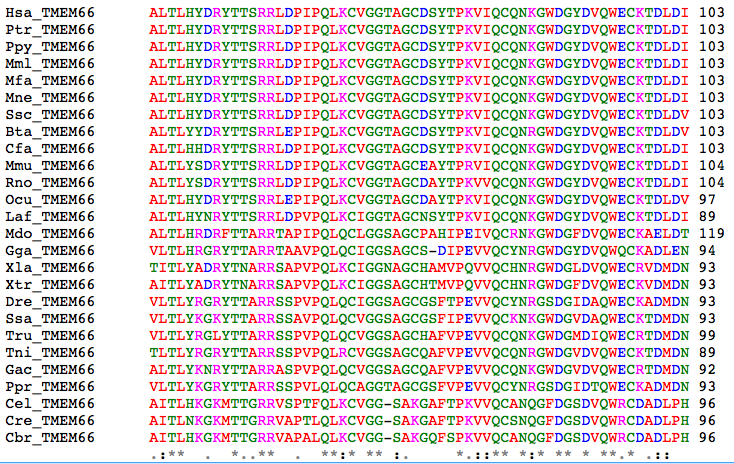
\includegraphics[scale=.5]{proteinalign}
\caption{An example of protein alignment \cite{proteins}}
\end{figure}

There are various computational algorithms that can be used to solve sequence alignment including slower but more accurate dynamic programming algorithms and faster but less accurate probabilistic or heuristic-based algorithms. In my work, it makes more sense to use the slower but more accurate methods, as our datasets are not so large and small mistakes that might be permissible to overlook in larger data could be much more egregious in smaller contexts.

The specific algorithm I chose to implement for solving the musical sequence alignment problem is a version of the Needleman-Wunsch dynamic programming algorithm for global sequence alignment. \footnote{This algorithm has a history of multiple invention. Needleman-Wunsch was first published in the context of protein alignment in bioinformatics. People with a more theoretical computer science bent might know the same algorithm by a different name, Wagner-Fisher.} 

At a high level, the Needleman-Wunsch algorithm and its family of dynamic programming sequence alignment algorithms calculate the edit distance between two sequences by producing a least-cost alignment of the sequences. An alignment is an assignment of pairwise characters and edit operations. Overall cost of an alignment (i.e. its \textbf{edit distance}) is determined by summing the individual costs of insertion, deletion, substitution, or no-change operations between pairwise characters in order to morph one sequence into the other. 

The next sections discuss coming up with edit distance calculations and then the method that Needleman-Wunsch uses to find the best alignment. 

\subsubsection{Edit Distance}

The term edit distance is a way of quantifying how dissimilar two sequences are to each other. If you think of sequences as being made up of characters, you can also think of one sequence transforming into the other through a series of insertion, deletion, substitution, and no-change operations, with each operation ''costing'' a certain amount. Edit distance is the smallest possible total cost associated with the transformation that is a series of operations that turns one sequence into another. As an example, consider the calculation of the edit distance between the two strings \textbf{MUSICAL} and \textbf{JUSTICE} that uses this series of operations for transforming \textbf{MUSICAL} into \textbf{JUSTICE}:

\begin{enumerate}
\item M $\rightarrow$  J (substitution)
\item $\epsilon \rightarrow$  T (insertion)
\item A $\rightarrow$  E (substitution)
\item L $\rightarrow  \epsilon$ (deletion)
\end{enumerate}


Note that implicitly I am excluding all the no-change operations that look like this:
\begin{enumerate}
\item U $\rightarrow$  U (no-change)
\end{enumerate}

\begin{table}[!h]
\centering
\begin{tabular}{ll}
\textbf{Operation} & \textbf{Cost} \\
Insertion          & 1             \\
Deletion           & 1             \\
Substitution       & 1             \\
No-change          & 0            
\end{tabular}
\caption{Naive Operation Cost Function Table}
\label{tab:naivetable}
\end{table}
	
This corresponds to an alignment that looks like figure \ref{best-alignment}. The green pair of characters indicate an insertion operation, red is deletion, and purple is substitution. These colors are also used in the visualization of OMR/MIDI stream alignment. 

\begin{figure}[!h]
\centering
\begin{tabular}{lcccccccccccc}
seq1 & {\color[HTML]{6200C9} \textbf{M}} & \textbf{U} & \textbf{S} & {\color[HTML]{009901} \textbf{\_}} & \textbf{I} & \textbf{C} & {\color[HTML]{6200C9} \textbf{A}} & {\color[HTML]{9A0000} \textbf{L}}  & \textbf{} & \textbf{} & \textbf{} &  \\
seq2 & {\color[HTML]{6200C9} \textbf{J}} & \textbf{U} & \textbf{S} & {\color[HTML]{009901} \textbf{T}}  & \textbf{I} & \textbf{C} & {\color[HTML]{6200C9} \textbf{E}} & {\color[HTML]{9A0000} \textbf{\_}} & \textbf{} & \textbf{} & \textbf{} & 
\end{tabular}
\caption{Alignment of MUSICAL and JUSTICE}
\label{best-alignment}
\end{figure}

The two strings have an edit distance of 4, because it requires four operations to completely morph one string into the other (discounting no-change operations).

However, one also might think that a substitution should ``cost'' more than either an insertion or deletion; after all, a substitution can be thought of as a consecutive insertion and deletion operation. 

A slightly different cost function that assigns more cost to substitution changes could look like table \ref{tab:naivetable2}. Using this cost function, the edit distance of changing \textbf{MUSICAL} into \textbf{JUSTICE} is 5.
\begin{table}[!h]
\centering
\begin{tabular}{ll}
\textbf{Operation} & \textbf{Cost} \\
Insertion          & 1             \\
Deletion           & 1             \\
Substitution       & 1.5             \\
No-change          & 0            
\end{tabular}
\caption{Operation Cost Table With Costlier Substitutions}
\label{tab:naivetable2}
\end{table}

But wait, should we certain subtypes of a single type of operation have differently weights? Consider if you were trying to run a spell checker (one application of string alignment and correction algorithms) on a word that wasn't recognized by the dictionary. In your particular spell check model, perhaps substitution of a vowel for a vowel isn't as costly as any other types of substitution. Let's say that substituting a vowel for a vowel should only have a cost of 1.2. Using this new cost function, the new edit distance is 4.7.
\begin{table}[!h]
\centering
\begin{tabular}{ll}
\textbf{Operation}             & \textbf{Cost} \\
Insertion                      & 1             \\
Deletion                       & 1             \\
Substitution - vowel for vowel & 1.2           \\
Substitution - all others      & 1.5           \\
No-change                      & 0                
\end{tabular}
\caption{Operation Cost Table With Different Substitution Costs}
\label{my-label3}
\end{table}

Considerations such as these go into the creation of a musical sequence aligner as well. 
\subsubsection{Alignment}

Recall that the edit distance between two sequences come from the least-cost alignment. The figure below shows a valid alignment, but it is certainly not the least-cost alignment, and therefore does not correspond to the edit distance between between the two sequences. 

\begin{figure}[!h]
\centering
\begin{tabular}{lcccccccccccc}
seq1 & {\color[HTML]{009901} \textbf{\_}} & {\color[HTML]{6200C9} \textbf{M}} & {\color[HTML]{6200C9} \textbf{U}} & {\color[HTML]{6200C9} \textbf{S}} & \textbf{I} & \textbf{C} & {\color[HTML]{6200C9} \textbf{A}} & {\color[HTML]{9A0000} \textbf{L}}  & \textbf{} & \textbf{} & \textbf{} &  \\
seq2 & {\color[HTML]{009901} \textbf{J}}  & {\color[HTML]{6200C9} \textbf{U}} & {\color[HTML]{6200C9} \textbf{S}} & {\color[HTML]{6200C9} \textbf{T}} & \textbf{I} & \textbf{C} & {\color[HTML]{6200C9} \textbf{E}} & {\color[HTML]{9A0000} \textbf{\_}} & \textbf{} & \textbf{} & \textbf{} & 
\end{tabular}
\caption{A bad alignment of MUSICAL and JUSTICE}
\label{badalign}
\end{figure}

If we have two sequences, of length $n$ and $m$, then we have $\binom{n+m}{m}$ possible alignments. Put into context, consider a two melodies of 10 notes each. Naively aligning just the note pitches, we have 184,765 different possible alignments! Clearly this isn't scalable, which is why we rely heavily on this piece of insight: A globally optimal alignment contains locally optimal alignments! This means that we can reuse the computations of subproblems to solve larger problems. What follows from this piece of insight is that for two strings split at $(i, j)$, the best alignment is:

\begin{center}
best alignment of \texttt{string1}$[:i]$ and \texttt{string2}$[:j]$ 
$+$ best alignment of \texttt{string1}$[i:]$ and \texttt{string2}$[j:]$
\end{center}

\begin{figure}[!h]`
\centering
\begin{tabular}{lccccccc}
   & {\color[HTML]{333333} \textbf{}} & \multicolumn{2}{c}{{\color[HTML]{333333} $i$}}          & {\color[HTML]{333333} \textbf{}} & {\color[HTML]{333333} \textbf{}} & {\color[HTML]{333333} \textbf{}} & {\color[HTML]{333333} \textbf{}} \\
   & {\color[HTML]{333333} \textbf{}} & \multicolumn{2}{c}{{\color[HTML]{333333} $\downarrow$}} & {\color[HTML]{333333} \textbf{}} & {\color[HTML]{333333} \textbf{}} & {\color[HTML]{333333} \textbf{}} & {\color[HTML]{333333} \textbf{}} \\
\texttt{seq1} & \textbf{M}                       & \textbf{U}                  & \textbf{S}                & \textbf{I}                       & \textbf{C}                       & \textbf{A}                       & \textbf{L}                       \\
\texttt{seq2} & \textbf{J}                       & \textbf{U}                  & \textbf{S}                & \textbf{T}                       & \textbf{I}                       & \textbf{C}                       & \textbf{E}                       \\
   &                                  &                             &                           &                                  & \multicolumn{2}{c}{$\uparrow$}                                      &                                  \\
   &                                  &                             &                           &                                  & \multicolumn{2}{c}{$j$}                                             &                                 
\end{tabular}
\caption{The alignment of MUSICAL split at \textit{i} and JUSTICE split at \textit{j}}
\label{indexed musical and justice}
\end{figure}

If we can keep track of all the possible alignment subproblems, we can recursively build an optimal solution using the answers from the subproblems. One way to represent this is with a scoring matrix indexed by $i$ and $j$. For the problem of aligning \textbf{MUSICAL} and \textbf{JUSTICE}, the setup would look something like this:


\begin{figure}[!h]
\centering
\begin{tabular}{lllllllll}
                                & \multicolumn{1}{c}{\textbf{-}} & \textbf{J}            & \textbf{U}            & \textbf{S}            & \textbf{T}            & \textbf{I}            & \textbf{C}            & \textbf{E}            \\ \cline{2-9} 
\multicolumn{1}{c|}{\textbf{-}} & \multicolumn{1}{l|}{}          & \multicolumn{1}{l|}{} & \multicolumn{1}{l|}{} & \multicolumn{1}{l|}{} & \multicolumn{1}{l|}{} & \multicolumn{1}{l|}{} & \multicolumn{1}{l|}{} & \multicolumn{1}{l|}{} \\ \cline{2-9} 
\multicolumn{1}{l|}{\textbf{M}} & \multicolumn{1}{l|}{}          & \multicolumn{1}{l|}{} & \multicolumn{1}{l|}{} & \multicolumn{1}{l|}{} & \multicolumn{1}{l|}{} & \multicolumn{1}{l|}{} & \multicolumn{1}{l|}{} & \multicolumn{1}{l|}{} \\ \cline{2-9} 
\multicolumn{1}{l|}{\textbf{U}} & \multicolumn{1}{l|}{}          & \multicolumn{1}{l|}{} & \multicolumn{1}{l|}{} & \multicolumn{1}{l|}{} & \multicolumn{1}{l|}{} & \multicolumn{1}{l|}{} & \multicolumn{1}{l|}{} & \multicolumn{1}{l|}{} \\ \cline{2-9} 
\multicolumn{1}{l|}{\textbf{S}} & \multicolumn{1}{l|}{}          & \multicolumn{1}{l|}{} & \multicolumn{1}{l|}{} & \multicolumn{1}{l|}{} & \multicolumn{1}{l|}{} & \multicolumn{1}{l|}{} & \multicolumn{1}{l|}{} & \multicolumn{1}{l|}{} \\ \cline{2-9} 
\multicolumn{1}{l|}{\textbf{I}} & \multicolumn{1}{l|}{}          & \multicolumn{1}{l|}{} & \multicolumn{1}{l|}{} & \multicolumn{1}{l|}{} & \multicolumn{1}{l|}{} & \multicolumn{1}{l|}{} & \multicolumn{1}{l|}{} & \multicolumn{1}{l|}{} \\ \cline{2-9} 
\multicolumn{1}{l|}{\textbf{C}} & \multicolumn{1}{l|}{}          & \multicolumn{1}{l|}{} & \multicolumn{1}{l|}{} & \multicolumn{1}{l|}{} & \multicolumn{1}{l|}{} & \multicolumn{1}{l|}{} & \multicolumn{1}{l|}{} & \multicolumn{1}{l|}{} \\ \cline{2-9} 
\multicolumn{1}{l|}{\textbf{A}} & \multicolumn{1}{l|}{}          & \multicolumn{1}{l|}{} & \multicolumn{1}{l|}{} & \multicolumn{1}{l|}{} & \multicolumn{1}{l|}{} & \multicolumn{1}{l|}{} & \multicolumn{1}{l|}{} & \multicolumn{1}{l|}{} \\ \cline{2-9} 
\multicolumn{1}{l|}{\textbf{L}}   & \multicolumn{1}{l|}{}          & \multicolumn{1}{l|}{} & \multicolumn{1}{l|}{} & \multicolumn{1}{l|}{} & \multicolumn{1}{l|}{} & \multicolumn{1}{l|}{} & \multicolumn{1}{l|}{} & \multicolumn{1}{l|}{} \\ \cline{2-9} 
\end{tabular}
\caption{Initial distance matrix setup for aligning MUSICAL and JUSTICE}
\label{alignsetup}
\end{figure}

Recall that we have defined the problem in three different ways:
\begin{enumerate}
\item Aligning \textbf{MUSICAL} and \textbf{JUSTICE}
\item Finding the edit distance between \textbf{MUSICAL} and \textbf{JUSTICE}
\item Finding a series of operations that transforms \textbf{MUSICAL} into \textbf{JUSTICE}
\end{enumerate}

All of these problem definitions are (almost) one and the same. Calculating the edit distance will also provide a good alignment of the two words and a good alignment necessitates a series of character change operations. It is important to know that that (3) has an implicit directionality built into the problem statement. It won't always be the case that alignments and transformations are symmetric (i.e. cost the same and have the same series of operations), and having a simple cost operation functions, such as in tables 
\ref{tab:naivetable}
 and 
 \ref{tab:naivetable2} 
 will make such problems symmetric. 

In this particular sample problem, we will always be transforming \textbf{MUSICAL} into \textbf{JUSTICE}. In the context of my thesis, we will always be transforming OMR sequences in MIDI sequences. 

After we've set up is the scoring matrix, we will populate it with initial values: 
\begin{enumerate}
\item 0 in $(0,0)$
\item $i-1 \cdot insertion cost$ for $i$ in $(i, 0)$ (this is the first column) 
\item $j-1 \cdot deletion cost$ for $j$ in $(0, j)$ (this is the first column) 
\end{enumerate}
[[somehow there needs to be an explanation that insertions are vertical movements, deletions are horizontal movements, and this is all relative to how you define the problem of transforming X->Y or Y->X ]]

After we've set up the initial matrix, we can go through and fill in all of the remaining slots using this update rule:


\begin{equation*}
\begin{split}
\text{D[i][j]} = &  \text{min \{ }\\
& \text{D[i-1][j] + insCost,} \\
& \text{D[i][j-1] + delCost,} \\
& \text{D[i-1][j-1] + subCost} \\
\text{\}}
\end{split}
\end{equation*}


\section{Turning Sequence Alignment into a Musical Problem}
Finding the edit distance of a musical sequence as opposed to a string of ASCII characters is a little trickier. First, there isn?t an intuitive ''space'' of music elements the way that there is a ''space'' of all characters. Second, even after identifying the musical elements, there isn?t an intuitive metric of distance between elements. For example, how would the distance between [Ab quarter note, 4th octave] and [Bb quarter note, 4th octave] compare with [Ab either note, 4th octave] and [Ab quarter note, 4th octave]? [pictures, maybe an even more ambiguous example]

Going back to [original model] and the questions we posed and answered for string alignment, 

\begin{itemize}
\item What sequences are and what makes them up: We can think of musical sequences as an ordering of notes, rests, and chords
\item The space that sequences occupy: This question can roughly be approximated as, what properties of notes, rests, chords do we care about? Some immediate answers are pitch, duration, rhythm.
\item Coming up with an appropriate metric for finding distance: In the previous section we had two different substitution functions. What kind of and how many ways do we want to calculate distance in musical elements?
\end {itemize}


\section{Related Work}
\subsection{Typke: Music Retrieval based on Melodic Similarity}
Another instance in which music is transformed and compressed into its most relevant features before comparison is in Typke's thesis on Music Retrieval based on Melodic Similarity \cite{typke}. Here, Typke proposes encoding music into what he calls a ``weighted point set" in a two-dimensional space of time and pitch before measuring any sort of melodic similarity between music. A note in a piece is represented as point set of pitch (in the Hewlett 40 system \cite{typke}) and an offset in quarter notes from the beginning of the piece.

\subsection{Church and Cuthbert: Rhythmic Comparison and Alignment}
Church and Cuthbert \cite{church} describe a system that hashes scores purely on rhythm and uses heuristics of rhythm in music (e.g. a repeated rhythm should be the same every time it is expected to repeat) to correct OMR scores. I believe that this model could be built upon with the hasher object in tandem with more heuristics pertaining to the qualities of music that I hash to further improve OMR accuracy.

\subsection{Viro: Peachnote, Musical Score Search and Analysis and IMSLP}
Peachnote \cite{peachnote} and IMSLP \cite{imslp} both are projects that contain large bodies of musical scores. Peachnote performs a search of a musical phrase and tends to introduce errors in chord progression searches that requires recognition of musical staves. IMSLP holds a large collection of musical scores. many of which are user contributed (i.e. not necessarily ground truth). Both of these bodies of work contain information about musical scores that my work can draw upon and use. 

\subsection{White: Statistical Properties of Music and MIDI}
White's dissertation \cite{white} describes properties of music that can be turned into heuristics for refining algorithmic analysis of music. Specifically, he builds upon Temperley's 1997 \cite{temperley} paper's details to harmonic analysis of MIDI and refers to other research that has been constructive towards Temperley's model. White does say that Temperley's algorithm fails when faced with ambiguity, such as in MIDI differentiating between enharmonic tones. The hope is that by combining the ambiguous parts of MIDI with the probabilistic and rigorous details of OMR scores, ambiguities in MIDI tonality can be resolved. In addition, White also cites a large repository of high quality MIDI files. 

\subsection{Rebelo et al: Optical Music Recognition - State-of-the-Art and Open Issues}
Rebelo et al's paper discusses the state of the art of OMR at each step of the OMR process and proposes future work in certain areas that would advance the current state of OMR. 
\cite{rebelo}

\subsection{OpenScore}
OpenScore is project
\chapter{Previous Work}
This chapter discusses previous work in musical sequence representation, alignment, and correction. The first half of the chapter is about work by others. The second half is my own previous work that was relevant to this thesis. 

\section{Related Work by Others}
In this section of work by others, 
\subsection{Typke: Music Retrieval based on Melodic Similarity}
Typke's thesis on Music Retrieval based on Melodic Similarity gives an example of how music can be transformed and compressed into its most relevant features \cite{typke}. Here, Typke proposes encoding music into what he calls a ``weighted point set" in a two-dimensional space of time and pitch before measuring any sort of melodic similarity between music. A note in a piece is represented as point set of pitch (in the Hewlett 40 system \cite{hewlett}) and an offset in quarter notes from the beginning of the piece. This representation allows for notes to be easily compared with each other. Since the features of notes are represented as numbers, it is convenient to do numerical operations with the representations. 

\subsection{Church and Cuthbert: Rhythmic Comparison and Alignment}
Church and Cuthbert \cite{church} describe a system that hashes scores purely on rhythm and uses heuristics of rhythm in music (e.g. a repeated rhythm should be the same every time it is expected to repeat) to correct OMR scores. This model was the original inspiration for building an alignment system with more heuristics pertaining to the qualities of music beyond just rhythm to further improve OMR accuracy.

\subsection{IMSLP}
IMSLP holds a large collection of musical scores (currently over 350,000), many of which are user contributed (i.e. not necessarily verified correct) \cite{imslp}. However, its contents are free and in the public domain. My work makes use of this large dataset. 

\subsection{Viro: Peachnote, Musical Score Search and Analysis}
Peachnote \cite{peachnote} is a project that contains a large bodyof musical scores. Peachnote performs OMR over the PDF scores in IMSLP and indexes the data for efficient querying and searching.  

\subsection{White: Statistical Properties of Music and MIDI}
White's dissertation \cite{white} describes properties of music that can be turned into heuristics for refining algorithmic analysis of music. Specifically, he builds upon Temperley's 1997 \cite{temperley} paper's details of harmonic analysis of MIDI and refers to other research that has been constructive towards Temperley's model. White does say that Temperley's algorithm fails when faced with ambiguity, such as in MIDI differentiating between enharmonic tones. The hope is that by combining the ambiguous parts of MIDI with the probabilistic and rigorous details of OMR scores, ambiguities in MIDI tonality can be resolved. In addition, White also cites a large repository of high quality MIDI files. 

\subsection{Rebelo et al: Optical Music Recognition - State-of-the-Art and Open Issues}
Rebelo et al's paper discusses the state of the art of OMR at each step of the OMR process and proposes future work in certain areas that would advance the current state of OMR \cite{rebelo}.

\subsection{OpenScore}
OpenScore is a project that aims to liberate all public domain music using both human and computer-powered techniques. Many works in the public domain are of low quality and/or are in formats that do not lend well to analysis, sharing, or reproducing, and OpenScore plans to turn them into high-quality music in digital formats. Both humans and computer software can aid in any part of the process, from transcription to error correction. The work of my thesis can directly contribute to the computer software tools that OpenSource is looking for. 

\subsection{\texttt{music21}}
\texttt{music21} is a open source Python library that is a toolkit for computer-aided musicology. It provides both a framework for representation of music as well as tools to perform analyses on music. The rhythm correctors built by Church and Cuthbert were made using the tools that \texttt{music21} provides. The work of my thesis relies heavily on the infrastructure of\texttt{music21}, its score and stream representations and their operations. 

\section{Previous Work: A Modular Universal Hasher} \label{hasher}
The work of my thesis uses the universal \texttt{Hasher} for digital representations of music tool. This work was largely done in the Spring of 2015 as part of my undergraduate capstone supervised independent study (6.UAP). 

Prior to my work on building a musical sequence aligner and fixer, I built a hasher with the specific intention that it would be able  to adapt according to different specification settings decided by the programmer. The programmer decides which kinds of \texttt{music21} stream elements, such as notes and chords, and properties, such as pitch name or duration, are relevant to their hash, and selects them to build a specific instance of a \texttt{Hasher} object. This \texttt{Hasher} instance can then be used to produce a hash from any \texttt{music21} stream. 

\subsection{Why Musical Comparison and Alignment Needs a Modular Hashing Function}
A hash function maps pieces of data of arbitrary size into data of fixed size and standard representation. If musical sequences could be discretized into elements and if these elements could be hashed, then the processes of comparison and alignment could be made deterministic and quick. 

Depending upon the problem statement that calls for a hash in the first place, this is a two step process:
\begin{enumerate}
\item discretizing a musical sequence into a list of relevant elements
\item hashing those elements  
\end{enumerate}
The details of this process can vary.  For instance, in determining the rhythmic similarity between two musical sequences, only the musical elements with durations (e.g. notes, chords, rests) in each sequence would be relevant. In hashing these elements, only properties such as duration and offset might be relevant. 

\begin{figure}[H]
\centering
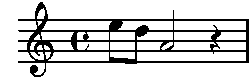
\includegraphics[scale=.7]{alg}
\caption[Rhythmic hash of a short melody]{
The hash of rhythmic features of this short melody would be \textit{NoteHash(offset=0, duration=0.5), NoteHash(offset=0.5, duration=0.5), NoteHash(offset=1.0, duration=2.0) NoteHash(offset=4, duration=1.0)}}
\end{figure}

As another example, in determining whether one piece is an approximate transposition of another, only the elements with some relation pitch (e.g. notes and chords) might be relevant.

\begin{figure}[H]
\centering
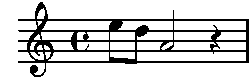
\includegraphics[scale=.7]{alg}
\caption[Melody transposition hash]{The hash of features related to transposition of this short melody would be \textit{NoteHash(intervalFromLastNote=0), NoteHash(intervalFromLastNote=-2), NoteHash(intervalFromLastNote=-5)}}
\end{figure}
Once a musical sequence is discretized and represented as a sequence of \texttt{NoteHash} objects, each individual tuple in the hash sequence can be thought of as a point in the space of all combinations of possible element properties. Then, canonical edit distance or string alignment algorithms can then be used to come up with a measure of similarity or an alignment between the two original musical sequences.

\subsection{Previous Work on Modular Hashing Functions}
The idea of extracting qualities of music specific to the needs of distance analyses and encoding that information in a lower-dimensional representation is not new. Typke in his thesis proposes what he calls a weighted point set representation of music \cite{typke}. His method of creating a weighted point set for a stream of music involves only taking melodic information (i.e. notes) and representing each discrete note as a three-tuple of (time, pitch, weight). The time component encodes information about the note's offset from the beginning. The pitch component encodes the note's pitch using the Hewlett's base-40 system (this is a numerical encoding similar to MIDI pitch but is also able to encode more information than just absolute frequency). The weight component is an assignment of how important the particular note is to the melody of the music stream." as something like "The weight component is an assignment of a numerical value to each note in the music stream, indicating the relative importance of the different notes within the melody \cite{hewlett}. 

\subsection{Overview of System}
The \texttt{Hasher} object is found in \texttt{hasher.py}. Its purpose is to identify the relevant features of relevant elements in any music stream and to represent them in a hashed format that is easy to compute with. Relevant elements here means objects such as notes, rests, chords. Relevant features here means qualities of these elements such as pitch, duration, offset. I represent these qualities in the hash as lightweight integers, floats, and strings, which makes future computations such as comparisons, and numerical operations easy and fast. 

Upon instantiation, \texttt{Hasher} does not take in any parameters. After an instance of \texttt{Hasher} is created, however, the user can set specific parameters in the \texttt{Hasher} to fit their own needs. The user must specify which relevant stream elements (notes, rests, chords) should be hashed, as well as which relevant qualities of those elements should be hashed (pitch, duration, offset, etc.). 

After the hashing parameters are set, the user calls the \texttt{hashStream} method on a stream. This method strips the stream only to the relevant elements, creates a set of hash functions based on the user's selection of relevant element qualities, and individually hashes each element with the entire set of specified hashing functions. 

The \texttt{Hasher} will create either a \texttt{NoteHash} or a \texttt{NoteHashWithReference} object for each element and add it to the end of the \texttt{FinalHash} list. Both are tuples that hold the hashed qualities of a single stream element. The only difference is that a \texttt{NoteHashWithReference} stores a reference back to the original stream element. Even though this has a lot of overhead, it is necessary if ever the original streams need to referenced for context or if they need to be changed.

The output of the entire process is a list of  \texttt{NoteHash} or \texttt{NoteHashWithReference} objects, stored in \texttt{finalHash}.

\subsubsection{Pre-Hashing: High Level Hasher Settings}
There are several system-wide high level settings that must first be set before the \texttt{hashStream} method can be called.
\begin{itemize}
\item \texttt{includeReference} - By default this is set to \texttt{False}, but if set to \texttt{True}, each element hash will be stored in a \texttt{NoteHashWithReference} object that includes a reference to the original element in its original stream. For many purposes, having this reference is not necessary and takes up extra overhead, so it is set to \texttt{False} by default.

\item \texttt{validTypes} - This is a list of the types of stream elements should be hashed. By default this is \texttt{[note.Note, note.Rest, chord.Chord]} and can be changed to be any subset of those three stream elements.
\item \texttt{stateVars} - This is a dictionary that keeps track of state between consecutive hashes. By default it doesn't contain anything, but can be programmed to contain \textit{intervalFromLastNote} and \textit{KeySignature} during the later process of preprocessing the streams and setting the appropriate hashing functions if the user-set parameters call for their use. 

\item \texttt{hashingFunctions} - This is the dictionary that stores maps which hashing functions should be used to hash which qualities. For example, if the user chose to hash notes and their MIDI pitch values, then the dictionary value for the key \textit{Pitch} would be \textit{\_hashMIDIPitchName}, the name of the function that takes a note and returns its MIDI pitch. 
\end{itemize}

        \subsubsection{Pre-Hashing: Low Level General Settings}
        These settings affect more than one of notes, rests, chords.
        
                    \begin{itemize}
                    \item \texttt{\_hashOffset} - If \texttt{True}, this will include in the hash a number that is associated with the offset of a musical element from the beginning of the stream. 
                    \item \texttt{\_hashDuration} - If \texttt{True}, this will include in the hash a number that is associated with its duration (measured in a multiplier of \texttt{duration.quarterLength}) .
                    \item \texttt{\_roundDurationAndOffset} - This is a boolean for determining whether offsets and durations should be rounded. This is useful for files (e.g. MIDI recordings without rounding) where beginnings of notes, rests, and chords may not fall exactly on the beat (e.g. beat 2.985 instead of 3).
                    \item \texttt{granularity} - A number that determines how precisely we round. If duration and offset are rounded, they will be rounded to this granularity of beat division. For example, a granularity of 32 will round notes to the nearest \nth{32} beat division and no further.
                    \end{itemize}
        
        \subsubsection{Pre-Hashing: Low Level Note Settings}
                    \begin{itemize}
                    \item \texttt{\_hashPitch} and \texttt{\_hashMIDI} - These settings determine whether the pitch of a note will be hashed, and if it is, how it will be represented. If \texttt{\_hashMIDI} is \texttt{True}, then the MIDI pitch value is hashed. Otherwise, its name representation is hashed (e.g.``C\#\#''). This setting is useful depending upon whether the user would want to differentiate between B\# and C.
                    \item \texttt{\_hashOctave} - If \texttt{True}, this includes in the hash the number octave that a note is in. This could be useful for an envelope-like following of pitches. 
                    \item \texttt{\_hashIntervalFromLastNote} - If \texttt{True}, this returns a number corresponding to the interval between the current note and the last note when applicable. This setting is a useful alternative to hashing pitch when trying to identify transpositions of pieces.
                    \item \texttt{\_hashIsAccidental} - If \texttt{True}, this will return a boolean indicating whether the pitch of the hashed element is outside of the key signature. This setting is currently not fully supported. 
                    \end{itemize}
        \subsubsection{Pre-Hashing: Low Level Chord Hashing Settings}
        Chords can be thought of as multiple notes happening at the same time. In \texttt{music21}, chords are their own type of object that can be decomposed into \texttt{note} objects. In the hashing system, chords can be hashed as chords, or by their constituent notes.
                    \begin{itemize}
                    \item \texttt{\_hashPrimeFormString} - If \texttt{True}, this includes in the hash of chord a string representation of its prime form.
                    \item \texttt{\_hashChordNormalOrderString} - If \texttt{True}, this includes in the hash of a chord a string representation of its normal order. 
                    \end{itemize}
        \subsubsection{Hashing: \texttt{hashStream}}
        Once the settings of a \texttt{Hasher} instance have been set, we can call its \texttt{hashStream} method on any stream. The following sections describe the what happens within a single \texttt{hashStreams} call. 
        \subsubsection{Hashing: Setting up \texttt{ValidTypes} and \texttt{StateVars}}
        First, the method \texttt{setupValidTypesAndStateVars} is called to set up the state variables and the valid hashing types. Recall that by default \texttt{stateVars} is empty and \texttt{validTypes} is \texttt{[note.Note, note.Rest, chord.Chord]} (of course, the user has already had the option of changing \texttt{validTypes} to contain any subset of the default types). This method checks whether the user has set either of these two settings:
        \begin{enumerate}
        \item \texttt{hashIntervalFromLastNote} - if this is set, then \texttt{IntervalFromLastNote} is added to \texttt{stateVars} to keep track of it. 
        \item \texttt{hashIsAccidental} - if this is set, then \texttt{KeySignature} is added to \texttt{stateVars} to keep track of, and \texttt{key.KeySignature} is added to the list of \texttt{validTypes} to hash. 
        \end{enumerate}
        
        \subsection{Hashing: Preprocessing the Stream}
        The stream that the \texttt{hashStream} method acts upon is stripped of all note ties in the \texttt{preprocessStream} if the \texttt{stripTies} setting is \texttt{True}. Additionally, this method returns the stream in a generator form by calling \texttt{recurse} on the stream. 
        
        \subsubsection{Hashing: Creating a List of Elements to be Hashed}
        Next the \texttt{hashStream} method builds a list of elements that are to be hashed by filtering the recursed stream of any types that are not in \texttt{validTypes}. This is stored in \texttt{finalEltsToBeHashed}.
        
        \subsubsection{Hashing: Building a Set of Hashing Functions}
        The method \texttt{setupTupleList} is called, and it sets up \texttt{tupleList}, \texttt{hashingFunctions} and \texttt{tupleClass}, all related to each other. \texttt{tupleList} is a list of all the element properties that should be hashed. \texttt{hashingFunctions} is a dictionary of which hashing function should be used for each property. \texttt{tupleClass} is a \texttt{namedtuple} that is constructed ad hoc based on which properties are to be hashed. The ad hoc construction accommodates for the fact that different \texttt{Hasher} instances will contain different things to hash. 
        
        \subsubsection{Hashing: Creating a \texttt{NoteHash} for Every Element}
        For each of the elements in \texttt{finalEltsToBeHashed}, the \texttt{Hasher} hashes its relevant properties using the hashing function listed in \texttt{hashingFunctions}. It then creates a single \texttt{NoteHash} that stores all the hashed properties.
        
        \subsubsection{Hashing: Building \texttt{finalHash}}
        If \texttt{includeReference} is set to \texttt{False}, then each new \texttt{NoteHash} object is directly added to \texttt{finalHash}. If \texttt{includeReference} is \texttt{True}, then each \texttt{NoteHash} gets replaced with a \texttt{NoteHashWithReference} object that includes a reference to the original stream element, and that gets added to \texttt{finalHash} instead.
    
\section{Previous Work: Low-level Object Comparison Optimizations} \label{spaceoptimizations}
Work during the fall of 2015 focused on optimizing the comparison process with variable-length data. The underlying idea was that Python objects tend to have more overhead than C objects, and if comparison and alignment algorithms were going to be doing a lot of comparisons between \texttt{NoteHash} objects produced by the Hasher, then converting these Python objects into C objects of appropriate size could save a lot of time. Here, ``appropriate size'' refers to the idea that NoteHash objects with only a few hashed properties would correspond to smaller C objects, and \texttt{NoteHash} objects with more hashed properties would correspond to larger C objects. 

A smart implementation of the most efficient method, Yeti Levenshtein, already exists in C, so my work was to cleverly convert variable-length \texttt{NoteHash} Python objects to C objects to use the Yeti Levenshtein library, which I hoped would be faster than using any Python edit distance algorithm.

I observed that the speedup we gained in converting variable-length NoteHash Python objects to C objects to use this library was a negligible cost compared to the run time of the comparison algorithm. This empirical evidence suggested that massive parallelization and speedup of the comparison process is difficult and that optimizations in alignment would be the key to significant speedup.

Thus, I concluded that musical comparison was already near the boundaries of its optimization and my work turned to focus on creating a robust alignment algorithm, which is described in the next chapter.  
%% This is an example first chapter.  You should put chapter/appendix that you
%% write into a separate file, and add a line \include{yourfilename} to
%% main.tex, where `yourfilename.tex' is the name of the chapter/appendix file.
%% You can process specific files by typing their names in at the 
%% \files=
%% prompt when you run the file main.tex through LaTeX.
\chapter{Final Implementation}
This chapter describes the final implementation of the entire OMR/MIDI musical stream alignment and correction system. First there will be an overview of the entire system. Then, there will be discussion on the final implementation of each of the large modules that is divorced from the context of the \texttt{OMRMIDICorrector} class. Afterwards, I will present an example use case of the system. I will conclude with a discussion of design tradeoffs and choices that I made in implementing the system.

The final implementation of the OMR/MIDI musical stream alignment and correction system. can be found in \texttt{omrMidiCorrector.py}. The OMR system is a combination of one or more of each of the \texttt{Hasher}, \texttt{Aligner}, and \texttt{Fixer} modules with specific parameters set. 

The inputs to the system are two \texttt{music21} streams (one OMR, one MIDI). The output of the system is a corrected OMR stream. 

\section{OMRMIDICorrector}

\subsection{System Overview}
The entire system resides within the \texttt{OMRMIDICorrector} class in \texttt{omrMidiCorrector.py}. This class is initialized with a \texttt{midiStream}, an \texttt{omrStream} and an optional \texttt{Hasher}. The \texttt{Hasher} parameter is optional because the system provides a default \texttt{Hasher} with some all-purpose settings if no \texttt{Hasher} is passed in. The method \texttt{processRunner} is the main method of this class that preprocesses the streams, sets up the appropriate \texttt{Hasher}, and calls the aligning and fixing methods.

\begin{figure}[!h]
\centering
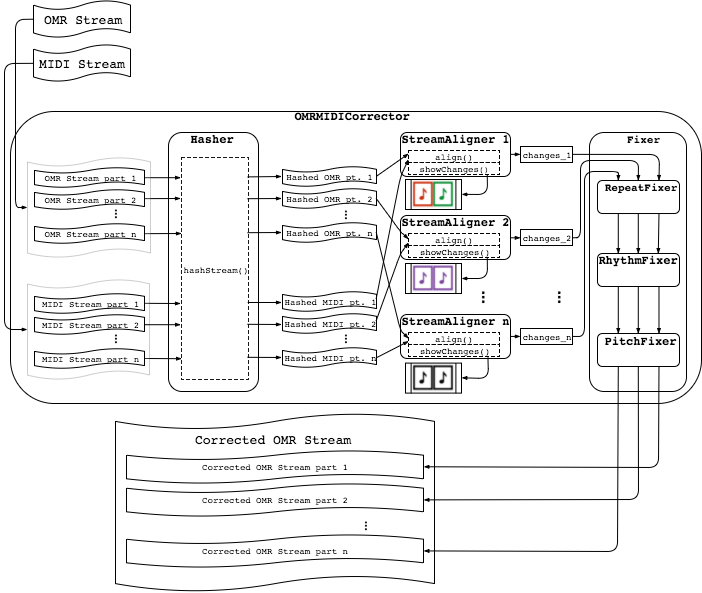
\includegraphics[width=\textwidth]{sysdiag10}
\caption{System diagram. The inputs to the system are OMR and MIDI streams. The output of the system is a corrected OMR stream.}
\end{figure}

\subsubsection{processRunner: preprocessStreams}
The \texttt{processRunner} first verifies the streams that are passed in and preprocess them before being hashed, aligned, and fixed in the method \texttt{preprocessStreams}

The first thing that \texttt{preprocessStreams} does is discretize the parts of the stream if the user has set \texttt{discretizeParts} to be \texttt{True}. Discretizing parts means to split the input streams into their constituent parts, so that the input streams are aligned part-wise. Since music is often comprised of multiple parts, this preprocessing step allows for input streams that contain nested streams. Take for example, an OMR/MIDI alignment of a string quartet. Both the OMR and MIDI inputs are stream in and of themselves, and so are all individual instrumental parts within both of the streams. 

A good alignment of the piece would involve aligning corresponding instrumental parts with each other to ensure that the beginnings and ends of corresponding parts aligned with each other. However, if we treat the inputs both as one long stream composed of four serial streams instead of four parallel streams, only the beginnings of the first instrumental parts and the ends of the last instrumental parts would be guaranteed to be aligned with each other. This guarantee comes from the global alignment method that I chose to implement. The figures below illustrate the phenomenon. 

\begin{figure}[!h]
\centering
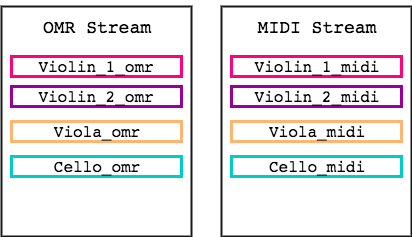
\includegraphics[width=.5\textwidth]{omrmidisheets2}
\caption{An example string quartet stream and its four parts.}
\vspace{10mm}
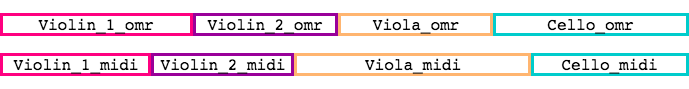
\includegraphics[width=.9\textwidth]{badalignstream2}
\caption{A bad alignment setup of the quartet would treat the entire piece as four serial streams and only the only guaranteed alignment would be between the beginning of the first part and the end of the last part.}
\vspace{10mm}
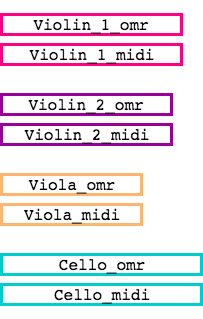
\includegraphics[width=.25\textwidth]{goodalignstream}
\caption{A better alignment setup of the quartet would do part-wise alignment instead of treating the entire piece as a sequence of parts. This methodology guarantees that the beginnings and ends of each part are aligned.}
\end{figure}

By default, \texttt{discretizeParts} is set to \texttt{True}. However, the user ultimately has the choice to align input streams part-wise or After a stream is split up into its constituent parts, the parts are stored in the lists \texttt{midiParts} and \texttt{omrParts}. The aligners and fixers work on all of the elements in the list, and so the entire system is agnostic to the number of parts; a stream comprised of a single part is processed in the same way as a multi-instrumental score. 

Then, \texttt{preprocessStreams} checks if the number of parts in MIDI and the OMR stream are the same. If they are off by more than one, then a \texttt{OMRMIDICorrectorException} is raised and the process halts. This is a cursory check to see if the two input streams can even reasonably be aligned.

If the numbers of parts are off by exactly one, then \texttt{preprocessStreams} spins up a lightweight \texttt{StreamAligner} object to try and see if there is an implicit bassline, where the bass doubles the cello part but an octave lower. In such a scenario, the OMR score would have one fewer part than the MIDI score because a bassist would read the cello line while reading sheet music, but the MIDI score would explicitly list all the instrument lines. If the similarity of the two streams is above a certain threshold, then I conclude that that bass part doubles the cello part and we disregard it in the alignment process. The \texttt{checkBassDoublesCello} method and its use of an \texttt{StreamAligner} object to determine whether two streams are an octave apart is a incidental example of a different use case of the \texttt{StreamAligner}.

\subsubsection{processRunner: setupHasher} \label{setuphasher}
The next step in the \texttt{processRunner} method is setting up the \texttt{Hasher} object that will be used to hash both input streams. This is done in the \texttt{setupHasher} method. If user has passed in a \texttt{Hasher} object upon instantiation of an \texttt{OMRMIDICorrector} object, then that is used. Otherwise this method sets up a default \texttt{Hasher} with settings we have found to be generally effective in the \texttt{setDefaultHasher} method. The default \texttt{Hasher} hashes only pitch and duration and includes references to the original stream elements. 

\subsubsection{processRunner: alignStreams}
This method creates a \texttt{StreamAligner} object for each pairwise MIDI part and OMR part found in \texttt{midiParts} and \texttt{omrParts} and aligns the two parts, calculates their similarity metrics, and visually shows the changes and alignment if \texttt{debugShow} is \texttt{True}. There is more detail about how the \texttt{StreamAligner} object works in section \ref{aligner}

\subsubsection{processRunner: fixStreams}
The last step is of the entire process is to fix the OMR stream. While the \texttt{Fixer} still remains in development, the description of this method and the \texttt{Fixer} in section \label{fixer} will remain at a high level. 

In its final implementation, \texttt{fixStreams} should create and instance of the \texttt{OMRMidiFixer} object. This would be a base class that does basic preprocessing on the \texttt{changes} list. All other fixers would extend from this class to fix a specific type of error in the original stream. The user would be able to choose which Fixers to apply to the original OMR stream.  

\section{Hasher}
The \texttt{Hasher} object used in the final implementation is a specific instance of the \texttt{Hasher} object described in section \ref{hasher}. The user can choose to pass in their own instance of \texttt{Hasher} or use the default \texttt{Hasher} provided.

\subsection{The Default Hasher}
The default \texttt{Hasher}, as described in section \ref{setuphasher}, hashes only pitch and duration of stream elements and set \texttt{includeReference} to be \texttt{True}. This setting is general enough to provide for a reasonable alignment for most generic alignment problems. But for more niche problems (for example, a rhythmic alignment), the user ought to define their own \texttt{Hasher} and the default \texttt{Hasher} should not be used. 

\subsection{NoteHashWithReference}
One update I made to the original \texttt{Hasher} was the addition of a new type of \texttt{NamedTuple} that includes a reference to the original element that is hashed and stored within the tuple. This new type provided access to the original stream elements which was necessary for three reasons:
\begin{enumerate}
\item It allows the user to visually see the alignment using the \texttt{showChanges} method in the \texttt{Aligner}. A list of the changes between two streams can be hard to parse and see patterns within, so this method provides a more visually appealing way of interpreting the list of changes.
\item It allows the user to access other elements in the context of the original stream element. For example, it might be helpful to be able to access the most recent key signature change in the stream for some fixing purpose. 
\item In order for the \texttt{Fixer} to fix the OMR stream, it must be able to change the original elements. 
\end{enumerate}

\section{Aligner} \label{aligner}
\subsection{System Overview}
\texttt{Aligner.py} contains the \texttt{StreamAligner} class that is the engine of the Alignment step. \texttt{StreamAligner} accepts as input two \texttt{music21} streams, one specified as a source stream, one as a target stream. The main functionality of \texttt{StreamAligner} is that it produces a global alignment between the source and the target streams in the form of a list of Change Tuples that maps each element in the source stream to an element in the target stream via one of the four change operations (insertion, deletion, substitution, no change). Additionally, \texttt{StreamAligner} also outputs a basic measurement of similarity between the two stream inputs \texttt{similarityScore}. Lastly \texttt{StreamAligner} has a \texttt{show} function that visually displays the alignment between the source and target streams. 

\subsection{Producing a Global Alignment}
The main objective of the Aligner is to produce a global alignment of two streams. In order to do so, it must hash the two streams with an instance of a \texttt{Hasher} (either passed in as a parameter during instantiation of a \texttt{StreamAligner} or using a default Hasher built into the \texttt{StreamAligner} class). After the two streams are hashed, \texttt{StreamAligner} sets up a distance matrix, a la the method described in Chapter 2 for classic string alignment, populates the matrix, and then performs a backtrace of the matrix starting the lower right corner to produce the alignment.

\subsubsection{Pre-Alignment: Setting Appropriate Parameters}
In the interest of being a modular system, I chose to give the programmer the option of setting their own Hasher. Upon instantiation of a \texttt{StreamAligner}, the programmer can choose to pass in an instance of a Hasher. If no Hasher is set initially, then \texttt{StreamAligner} uses the default Hasher that is set to hash Notes, Rests, and Chords, and their MIDI pitches and durations. The default Hasher is generic enough to be able to work with general alignment, but a more niche problem would require the programmer to use a Hasher more specific to their problem

I also chose to leave the cost of Insertion, Deletion, and Substitution easily substitutable as well. By default, the cost of both Insertion and Deletion is equal to the length of one of the \texttt{NoteHashWithReference} tuples, which is exactly the number of properties that are hashed of any musical element. (So in the case of the default Hasher, Insertion and Deletion both have cost 2.) The cost of Substitution between two \texttt{NoteHashWithReference} tuples is equal to the number of properties they don't have in common with each other. For example, the cost of substituting 
$$ \texttt{NoteHashWithReference(pitch=59, offset=1.0, duration=2.0)} $$
with either 
$$\texttt{NoteHashWithReference(pitch=59, offset=1.0, duration=3.0)} $$ or 
$$\texttt{NoteHashWithReference(pitch=60, offset=1.0, duration=2.0)} $$
would have a cost of 1. 

\subsubsection{Pre-Alignment: Hashing the Streams}
The alignment algorithm can only be applied after the streams are represented in a hashed format as a list of \texttt{NoteHashWithReference} tuples. Both input streams will be hashed and stored as the \texttt{hashedTargetStream} and the \texttt{hashedSourceStream}. The hashed format is the analog to a string and each \texttt{NoteHashWithReference} tuple is the analog to a character in classic string alignment.

It recommended that the hasher used to the hash the streams be set to include references to the original stream by using \texttt{NoteHashWithReference} tuples in the creation of the hash (as opposed to the \texttt{NoteHash} tuple that has much less overhead), and in the default hasher,  This ensures that the \texttt{show} function and future fixers have access to the original objects that each hash came from. This makes it easier to color the original objects in the case of the show function and to extract any necessary metadata that wasn't encoded in the hash for future fixers.

There is also an option to indicate that the streams passed in are already hashed, but in the context of my thesis work, this should never be the case. 

\subsubsection{Alignment: Initializing the Distance Matrix}
The first step in the alignment process is initializing the distance matrix. We set up an empty $n+1 \times m+1$ matrix, where $n$ is the length of the hashed target stream and the $m$ is the length of the hashed source. The extra column and extra row are populated with initial costs that correspond to just Insertion or just Deletion operations. In the leftmost column, the value $i \times insertCost$ is put into entries $(i, 0)$. In the topmost row, the value $j \times deleteCost$ is put into entries $(0, j)$. 

\subsubsection{Alignment: Populating the Distance Matrix}
The next step in the alignment process is to fill in the remainder of the distance matrix with values generated with these update rules. 

\begin{equation*}
\begin{split}
\text{D[i][j]} = &  \text{min \{ }\\
& \text{D[i-1][j] + insCost,} \\
& \text{D[i][j-1] + delCost,} \\
& \text{D[i-1][j-1] + subCost} \\
\text{\}}
\end{split}
\end{equation*}


where 
\begin{align*}
	\text{insCost = }  {}& \text{insertCost(hashedSourceStream[0])} \\
	\text{delCost = } {}& \text{deleteCost(hashedSourceStream[0])} \\ 
	\text{subCost = } {}& \text{substitutionCost(}  \text{hashedTargetStream[i-1]},  \-
	\text{hashedSourceStream[j-1])} \\						
\end{align*}

Each entry A[i][j] in the distance matrix stores the lowest cost for aligning\\
 \texttt{hashedTargetStream[i]} with \texttt{hashedSourceStream[j]}. There are 4 possible ways of relating the two tuples. 
\begin{enumerate}
\item \textit{\texttt{hashedTargetStream[i]} is an insertion} - in the case of insertion, the cost of aligning \texttt{hashedTargetStream[i]} with \texttt{hashedSourceStream[j]} is equal to the cost of aligning \texttt{hashedTargetStream[i-i]} with \texttt{hashedSourceStream[j]} plus the cost of insertion.

\item \textit{\texttt{hashedTargetStream[i]} is a deletion} - similar to the insertion case, for deletion, the cost of aligning \texttt{hashedTargetStream[i]} with \texttt{hashedSourceStream[j]} is equal to the cost of the subproblem of aligning \texttt{hashedTargetStream[i]}  with \texttt{hashedSourceStream[j-i]} plus the cost of deletion.

\item \textit{\texttt{hashedTargetStream[i]} is a substitution of \texttt{hashedSourceStream[j]}} - in the case of substitution, the cost of aligning \texttt{hashedTargetStream[i]} with \texttt{hashedSourceStream[j]} is equal to the cost of the subproblem of aligning \texttt{hashedTargetStream[i-i]} with \texttt{hashedSourceStream[j-1]} plus the cost of a substitution of  \texttt{hashedSourceStream[j]} for \texttt{hashedTargetStream[i]}.
 
\item \textit{No change between the two tuples i.e. the two tuples are the same} - same as above, where substitutionCost(\texttt{hashedTargetStream[i]}, \texttt{hashedSourceStream[j]}) is 0.
\end{enumerate}

The method \texttt{populateDistanceMatrix} fills in all the entries of the distance matrix using the rules and calculations listed above. It is important to note that in my work, all changes are made relative to \texttt{TargetStream}. That is, whenever possible, \texttt{SourceStream} is the stream that is being transformed into \texttt{TargetStream}. This invariant holds because in OMR/MIDI correction, the approach and direction I take is to change OMR into MIDI. Therefore, the MIDI stream is always the \texttt{TargetStream} and the OMR stream is always the \texttt{SourceStream}. It is certainly possible to go in either direction, but this paper will do it this way. 

\subsubsection{Alignment: Backtrace to Find the Best Alignment and Create the Changes List}
Once the distance matrix has been completely filled in, we use a backtrace starting from the bottom right hand corner of the matrix (i.e. A[i][j]) to find the path of least of cost. 

Starting from the value found at A[i][j], we look at the values directly above, to the left, and diagonal in the up-left direction. That is, we look at the values in A[i-][j], A[i][j-1], and A[i-1][j-1]. Among these three values, we choose the minimum value. The combination of direction and value that we moved in tells us what kind of operation was performed to align NoteHashWithReference tuples \texttt{hashedSourceStream[i]} and \texttt{hashedSourceStream[j]}:
\begin{enumerate}
\item if the direction is up, then regardless of the value, this corresponds to an insertion operation.
\item if the direction is left, then regardless of the value, this corresponds to an insertion operation.
\item if the direction is diagonal up-left, and the value at A[i-1][j-1] is \textit{different} from the value at A[i][j], then this corresponds to a substitution operation.
\item if the direction is diagonal up-left, and the value at A[i-1][j-1] is the \textit{same} as the value at A[i][j], then this corresponds to a no-change operation.
\end{enumerate}  

We continue this backtrace until we end up back at A[1][1]. Since we are using a global alignment technique, we should always end up back at this entry. If at the end of backtrace we end up in another part of the distance matrix, the method throws an \texttt{AlignmentException}. 

Additionally, at every step of the backtrace, we create a \texttt{ChangeTuple} that holds references to the original musical elements that are represented in the original \texttt{SourceStream} and \texttt{TargetStream} and the kind of operation (insertion, deletion, substitution, no-change) that links them. Then we insert this \texttt{ChangeTuple} into the beginning of the \texttt{changes} list.

This is all performed in the \texttt{calculateChangesList} method. 

\subsubsection{Post-Alignment: Measures of Similarity}
After the backtrace to find the alignment, there is enough data to calculate some basic metrics of similarity. 

\texttt{changesCount} is a Counter object that provides a count of how many of each of the four different change operations appear in the \texttt{changes} list. 

\texttt{similarityScore} is a float between 0 and 1.0 that is the ratio of \texttt{NoChange} operations to the total number operations in the \texttt{changes} list.
\subsubsection{Post-Alignment: Visual Display of Alignment}
The \texttt{showChanges} method provides a visual display of how the two streams are related via the \texttt{changes} list. For each \texttt{ChangeTuple} in the list, this method goes back to the initial reference and changes the color of the element in reference and adds in an id number as a lyric to that element if the change operation is not a \texttt{NoChange}. The color is determined by the type of change operation. Green corresponds to an insertion, red to deletion, and purple to substitution. The id number is the index of the \texttt{ChangeTuple} in the list. 

The figures below shows the visual display of alignment between a scanned score of an excerpt of \textit{String Quartet No.7 in E-flat major, K.160: I. Allegro} and a MIDI recording of the same piece as well as the original score that the OMR came from. 

\begin{figure}[!ht]
\centering
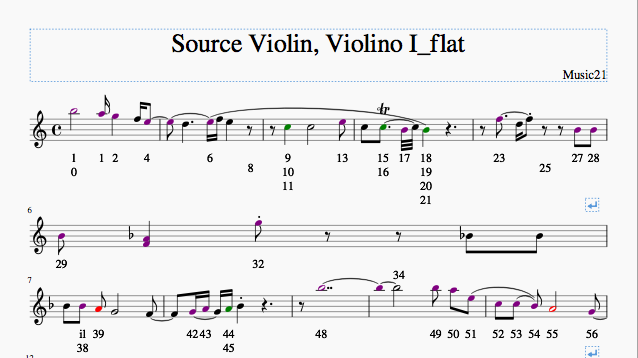
\includegraphics[width =.9\textwidth]{sourceshow}
\caption{Visual display of changes in source (OMR) stream}
\end{figure}

\begin{figure}[!ht]
\centering
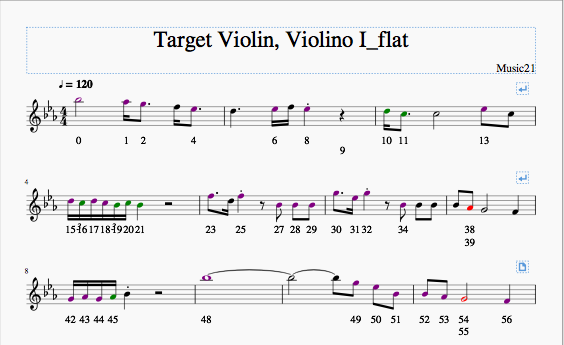
\includegraphics[width =.9\textwidth]{targetshow}
\caption{Visual display of changes in target (MIDI) stream}
\end{figure}

\begin{figure}[!ht]
\centering
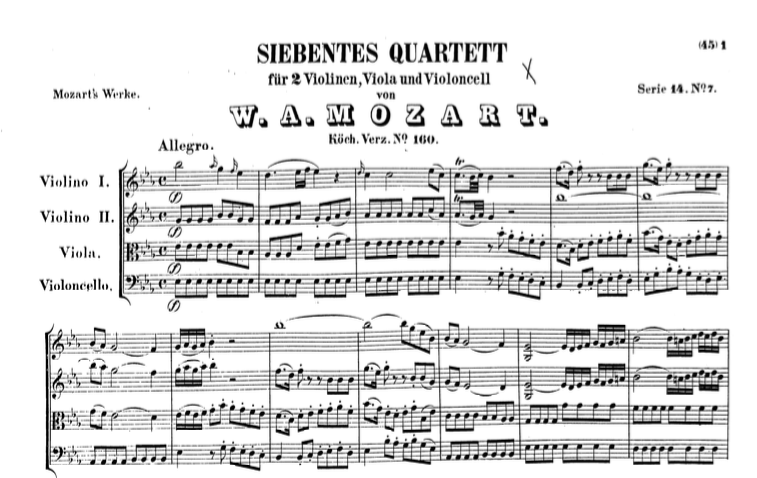
\includegraphics[width =.9\textwidth]{sourceomr}
\caption{Excerpt of original score taken from IMSLP}
\end{figure}

Since this method has a lot of overhead, it is by default set not to run. It can be set to run for every alignment by passing in the argument \texttt{show=True}. 

\section{Fixer} \label{fixer}
The \texttt{Fixer} is the last part of the OMR/MIDI music stream alignment and correction system. Its developmental work can be found in \texttt{fixer.py}. The high level idea is that there is a base class called \texttt{OMRMidiFixer} that takes as input the \texttt{changes} list that the \texttt{StreamAligners} outputs. It would also do basic preprocessing on the \texttt{changes} list, including dividing it up into \texttt{chunks}, substrings of the the \texttt{ChangeTuples} in the \texttt{changes} list that correspond to a small scale alignment of the corresponding stream elements in the original streams. 

Additional child Fixer classes would inherit from the parent \texttt{OMRMIDIFixer} class and correct very specific problems. For example, in the \texttt{StaccatoFixer} skeleton code, I have identified a pattern that \texttt{chunks} of \texttt{ChangeTuples} would exhibit that would indicate that the OMR process failed to recognize a passage that is marked as staccato. The \texttt{StaccatoFixer} class along with other children \texttt{Fixer} classes would look for similar patterns in the \texttt{ChangeTuples} list and correct the OMR stream based on this information. 

In section \ref{futurefixers} I discuss what I envision future \texttt{Fixers} to look like based on the groundwork I have laid out for the fixing process.

\section{Tradeoffs and Design Decisions}

In this section, I will justify some of my design choices and discuss tradeoffs in my decisions. 

\subsection{Modularity vs. Simplicity}
\subsubsection{A Variety of Settings and a Longer Setup}
All of the modules have many different settings with various parameters. The variety of settings is what makes the \texttt{Hasher} and \texttt{Aligner} so powerful--- by changing just a couple of settings, both are able to solve very different problems.

However, this necessarily lends itself to the system being more complex because each module must be able to handle various combinations of settings and their edge cases. It also requires the user to be careful when selecting initial settings. 

One alleviation to this problem is providing default settings to all the modules. These default settings are what I believe are good general settings for the most common uses of the modules. 

\subsubsection{Length Agnosticism}
There are two instances in which I purposefully built the system to be able to handle variable length input--- in building \texttt{NoteHash} and \texttt{NoteHashWithReference} tuples and in building the \texttt{OMRMIDICorrector} to be able to process a stream with any number of parts. Both of these decisions make the entire system more powerful because the system is able to process many more different types of streams this way, but it also makes the hashing and aligning process more convoluted. Fortunately for the user, all of this is hidden under the hood. There are likely some performance hits that are associated with this added complexity, but not to the point of inoperability. More demonstrations on timing are shown in section \ref{timing}.

\subsection{Performance vs. Space and Object Overhead}

\subsubsection{NoteHashWithReference}
The \texttt{NoteHashWithReference} object contains a reference to the original stream object. Streams and the elements they contain are complex objects, so \texttt{NoteHashWithReference} objects have much more overhead in storage than their counterparts, \texttt{NoteHash} objects. However, in setting up a \texttt{Hasher} object, the user has the decision to use either one.   

\subsubsection{Creating One Hasher and Many Aligners}
During the correction process, only a single \texttt{Hasher} object is created and used and reused to generate hashes for every part in the stream passed in. There was the option of having \texttt{Hasher} object be one-time-use objects, but I chose to have the \texttt{Hasher} be able to operate on multiple streams. 

On the other hand, a new \texttt{StreamAligner} object is generated for every pair of parts in the OMR and MIDI streams that are passed in. 

Between generating \texttt{NoteHashWithReference} objects for every hashed stream element and \texttt{StreamAligner} objects for every pair of streams, there is a lot of space overhead taken up in even just a single alignment and correction process. However, based on experimental findings in which I tried to create these objects in C, perform the comparisons in C, and then translate the results into Python, I concluded that the limiting factor of the process was not in Pythonic object creation but rather the comparison process that calculates Levenshtein edit distance. The results and findings are discussed in more detail in section \ref{spaceoptimizations}.


\subsection{Manual User Input}
The OMR and MIDI streams that are used as input to the system come from somewhere. I have left the onus on the user to source .mid files and find scanned scores. I also have left it to the user to use some kind of OMR tool to convert the scanned score and the MIDI file into a musicXML form. Once in musicXML form, the user can use the \texttt{music21} library to parse the OMR and MIDI and convert them into \texttt{music21} streams. 

I leave this as a task to the user instead of automating it because with practice, humans can be much more precise and efficient with this process, and the necessity of a (probably large and complicated) computer program to do the same thing decreases. 

\section{A Use Case}
%% This is an example first chapter.  You should put chapter/appendix that you
%% write into a separate file, and add a line \include{yourfilename} to
%% main.tex, where `yourfilename.tex' is the name of the chapter/appendix file.
%% You can process specific files by typing their names in at the 
%% \files=
%% prompt when you run the file main.tex through LaTeX.
\chapter{Examples and Results}
This chapter will describe the results of my work using an excerpt of of W. A. Mozart's \textit{Eine Kleine Nachtmusik, K.525- I.Allegro} (referred to by just ``K.525'' from here onwards) as an example. It will also use an excerpt of W. A. Mozart's \textit{String Quartet No.7 in E-flat major, K.160- I.Allegro} (referred to by just ``K.160'' from here onwards) as an example where K.525 doesn't fit the specifications. This chapter will also look at timing metrics of the system.

\section{Eine Kleine Nachtmusik, K.525- I.Allegro, W. A. Mozart}		
This section will go through an example of how the entire \texttt{OMRMIDICorrector} system works on W. A. Mozart's \textit{Eine Kleine Nachtmusik, K.525- I.Allegro}.

\begin{figure}[H]
\centering
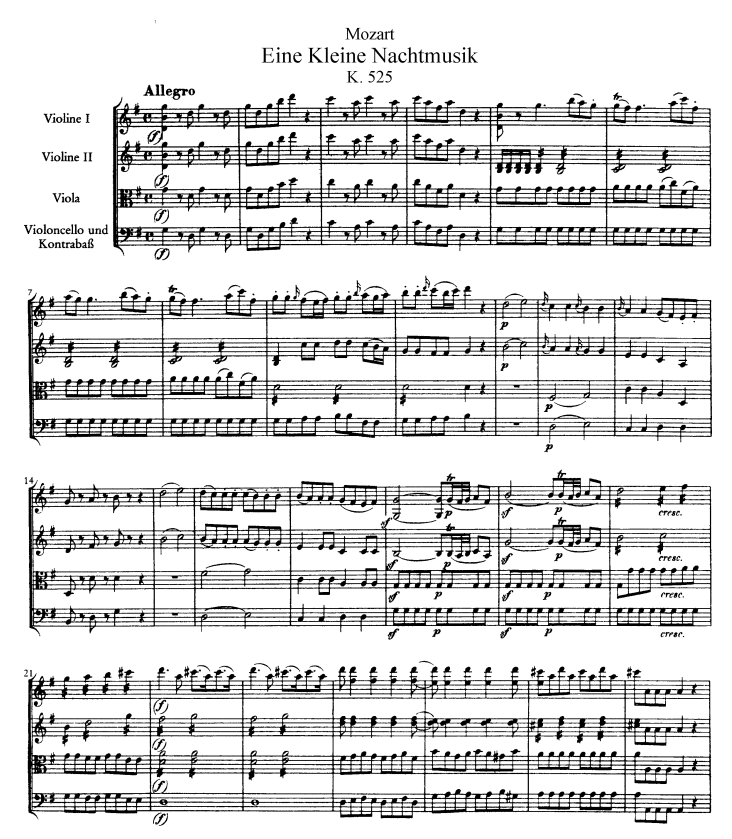
\includegraphics[width =.9\textwidth]{k525originalomrscan}
\caption{The first page of the scanned copy of the score found on IMSLP.}
\end{figure}

\subsection{Musical Properties of K.525}
I chose K.525 as the example piece for its many music properties that make it a difficult but interesting piece to align.

\subsubsection{Bass and Cello Doubling}
In the original scanned score, there are only four parts because the bass part doubles the cello part one octave lower. However, in the MIDI encoding, there are five separate voices. Thus, in the preprocessing step of the \texttt{OMRMiDICorrector}, it would be ideal for the system to recognize this. Otherwise, in instances where the \texttt{OMRMIDICorrector} could not pair up the parts between the input OMR stream and the input MIDI stream, there would be an error thrown, and alignment and correction would not happen. 

\subsubsection{Tremolos}
Starting in measure 5 in the original scanned score, the second violin has tremolo notes, instead of repeated \nth{16} notes written out. The OMR parser in SmartScore is not robust enough to recognize the slashes across the stem of the note as tremolo markings and instead interprets it as a single note. The MIDI protocol has no way of indicating tremolos, so the second violin's notes in measure 5 are encoded as regular \nth{16} notes. The \texttt{Aligner} is robust enough to align tremolo measures with non-tremolo measures even though there is a huge discrepancy in the number of notes present in the measure.

\subsection{Preparing the Raw Input}
The basic raw input of the system is an OMR score and a MIDI file. A scanned copy of the score was found in IMSLP \cite{k525}, the source for much free public domain sheet music. The MIDI file was sourced from the Yale MIDI Archive. 

I used SmartScore's built-in OMR tool to convert the scanned score of K.525 into an ENF file. Then I exported the post-OMR file as a musicXML file.

Similarly for the K.525 MIDI file, I used SmartScore to parse the original file and exported it as a musicXML file. 

The last step of preparing the raw input is to parse the musicXML files with the \texttt{music21} library so that they are \texttt{Stream} objects. This can be done by passing in the musicXML filepaths to the \texttt{parse} method in the \texttt{converter} class. We will call these two parsed streams \texttt{k525midiStream} and \texttt{k525omrStream}. 
\begin{minted}{python}
from music21 import *
k525MidiFilepath = "pathto/k525mvmt1/miditoxml.xml"
k525OmrFilepath= "pathto/k525mvmt1/omrtoxml.xml"
k525midistream = converter.parse(k525MidiFilepath)
k525omrstream = converter.parse(k525OmrFilepath)
\end{minted}
\subsection{Running \texttt{OMRMIDICorrector} on K.525}
After the raw input has been massaged into \texttt{Stream} objects, the aligning process is simple. We create an instance of an \texttt{OMRMIDICorrector} object with the two streams as parameters. For the purposes of this example, we will use the default hasher that is built into the \texttt{OMRMIDICorrector} class. We will set the \texttt{debugShow} to \texttt{True} so that we can visualize the alignment between pairwise streams. Finally, we will call \texttt{processRunner} which will hash and align the parts in the stream. For now, we will manually create the \texttt{Fixer} objects for stream fixing. The aligner is able to correctly identify that the repeated \nth{16} notes 

\begin{minted}{python}
from music21 import *
OMC = alpha.analysis.omrMidiCorrector
k525omc = OMC.OMRMIDICorrector(k525midistream, k525omrstream)
k525omc.debugShow = True
k525omc.processRunner()
\end{minted}

The outputs of the \texttt{showChanges} function are all in Appendix \ref{appb}

\subsubsection{A Closer Look at Specifics of \texttt{processrunner}}
A lot of magic happens within \texttt{processRunner}, all of which was described at a high level in sections \ref{processrunner1} - \ref{processrunner2}. Here are some salient details of the process in the context of K.525 that I think deserve notice:
\begin{itemize}
\item Bass Doubles Cello Part - The OMR score has only four parts, whereas the MIDI score has 5. The \texttt{checkBassDoublesCello} method in \texttt{OMRMIDICorrector} is able to correctly identify this and thus does not reject the input on the basis of having a mismatching number of parts in the stream. 
\item Rhythmic Fault Tolerance: Beginning Rests - The first measure in the OMR score is a scanning and parsing error. The \texttt{Aligner} is robust enough to identify the beginning rest as a insertion error. 
\item Rhythmic Fault Tolerance: Propagating Rhythmic Shifts - By measure 5 in the Violin 2 part, we see that the OMR score has introduced a \nth{16} note shift in the rhythm which continues for a few measures. 
\item Notation Fault Tolerance: Tremolos - By measure 5 of the Violin 2 part and by measure 10 of the Viola part, the repeated \nth{16} notes get notated with tremolo slashes in the original OMR score. Of course, the MIDI protocol doesn't have a way of representing tremolo, so the notes are written out in long form. The corrector is able to match the written out repeated notes in the MIDI to the (incorrectly) scanned corresponding notes in the OMR. 
\end{itemize}

\subsection{Example 1: Similarity Metrics in K.525}
Recall that the \texttt{similarityScore} is the ratio of \texttt{NoChange} operations to the total number of operations in the \texttt{changes} list. For each pair of streams in K.525, the \texttt{similarityScore} and \texttt{changesCount} are listed below:
\begin{table}[H]
\centering
\begin{tabular}{lll}
           & \texttt{similarityScore} & \texttt{changesCount}                                                  \\
Violin 1   & 0.51                       & \{NoChange: 83, Ins: 30, Del: 10, Sub: 39\} \\
Violin 2   & 0.30                       & \{NoChange: 74, Ins: 125, Del: 9, Sub: 38\} \\
Viola      & 0.72                       & \{NoChange: 97, Ins: 21, Del: 9, Sub: 8\}   \\
Cello/Bass & 0.87                       & \{NoChange: 107, Del: 11, Sub: 5\}               
\end{tabular}
\caption{\texttt{similarityScore} and \texttt{changesCount} for every pair of aligned streams}
\end{table}

A visual examination of the pairs of streams suggests that these numbers and counts look correct. The Cello/Bass parts have the fewest colorations to their notes and no insertion changes at all. The least similar pair of parts is the Violin 2, which has multiple cases of the tremolo problem described above as well as propagating rhythmic shifts.

\section{String Quartet No.7 in E-flat major, K.160- I.Allegro, W. A. Mozart}
The previous section showed the alignment between parts in \textit{Eine Kleine Nachtmusik}. In this section will use another piece by Mozart to demonstrate how the \texttt{EnharmonicFixer} works on correcting an excerpt of the Violin 1 part of K.160. This OMR score was also sourced from IMSLP \cite{k160}.

\subsection{Running \texttt{EnharmonicFixer} on K.160, Violin 1}
After prepping the raw input files of K.160 in the same way as detailed above and running that through an \texttt{OMRMIDICorrector} instance, we will create an \texttt{EnharmonicFixer} instance using just the Violin 1 OMR stream and MIDI stream and the associated \texttt{changes} list.

\begin{minted}{python}
from music21 import *
k160MidiFilepath = "pathto/k160mvmt1/miditoxml.xml"
k160OmrFilepath = "pathto/k160mvmt1/omrtoxml.xml"
         
k160midiStream = converter.parse(k160MidiFilepath)
k160omrStream = converter.parse(k160OmrFilepath)
k160omc = OMRMIDICorrector(k160midiStream, k160omrStream)
k160omc.processRunner()
        
V1Changes = k160omc.changes[0]
V1Midi = k160omc.midiParts[0]
V1Omr = k160omc.omrParts[0]
k160EF = fixer.EnharmonicFixer(V1Changes, V1Midi, V1Omr)
k160EF.fix()

k160omcViolin1OmrStream.show()
\end{minted}

In Appendix \ref{appc}, the first two figures show the alignment visualization of the Violin 1 part. The last figure shows the corrected OMR score after it has been changed by the \texttt{EnharmonicFixer}.

\subsection{Analysis of Correction}
Visual inspection of figures \ref{fig:k160postalignv1midi} and \ref{fig:k160postalignv1omr} suggests that the OMR failed to pick up the appropriate key signature of the movement and that is what lends to large number of changes in the first 10 or so measures. Inspection of figure \ref{fig:k160postfixv1} shows that many of the pitch errors have been corrected using the \texttt{EnharmonicFixer}. Of course, the most ideal scenario would be to recreate the key signature, but having the correct pitch is a good start. 

\section{Results: Timing Tests} \label{timing}
This section will evaluate the runtime on each of the three major modules of the system the \texttt{Hasher}, \texttt{Aligner}, and\texttt{Fixer} as well as the entire system, \texttt{OMRMIDICorrector} which is a combination of some number of instances of the three major modules. It will also discuss how the system would scale to different sized inputs. 

For the following calculations, assume that the length of the input MIDI stream and the OMR stream are about the same, $n$, and that the number of parts in each of the streams is $p$. 

\subsection{Runtime Analysis: \texttt{Hasher}}
Setup of the \texttt{Hasher} object is in $O(n)$ time. Building the list \texttt{finalEltsToBeHashed} requires scanning the input stream in full. Recall that the \texttt{tupleList} is a list of the stream element properties that will be hashed; call its length $t$. The runtime of the \texttt{hashStream} method is then $O(k \cdot n)$. 

Thus, a single use of the \texttt{Hasher} is in $O(n) + O(k \cdot n) = O(n)$ time for small $k$. This is a reasonable assumption because the number of notes in a stream is likely to be far greater than the number of possible qualities of stream elements that can be hashed. 

\subsection{Runtime Analysis: \texttt{Aligner}}
Setup of a \texttt{StreamAligner} object takes $O(n \cdot n) = O(n^2)$ time, dominated by the \texttt{populateDistanceMatrix} function. Traceback in the \texttt{calculateChangesList} method takes $O(n+ n) = O(n)$ time. The length of the \texttt{changes} list is then also $O(n)$. The runtime of \texttt{showChanges} is proportional to the length of the \texttt{changes} list, calculated above to be $O(n)$

A single use of a \texttt{StreamAligner} object is in $O(n^2) + O(n) +O(n) = O(n^2)$ time. 

\subsection{Runtime Analysis: \texttt{Fixer}}
The \texttt{OMRMIDIFixer} and the \texttt{EnharmonicFixer} both require negligible setup. The \texttt{fix} function's runtime is proportional to the length of the \texttt{changes} list input, shown above to be $O(n)$. 

A single use of a \texttt{Fixer} object is in $O(n)$ time. 

\subsection{Runtime Analysis: \texttt{OMRMIDICorrector}}
For a single instance of an \texttt{OMRMIDICorrector} with OMR and MIDI streams of length $n$ and $p$ parts, there are $2 \cdot p$ texttt{Hasher} objects, $p$ \texttt{Aligner} objects, and $p$ \texttt{Fixer} objects created. In total this comes out to a time of:
$$2 \cdot p \cdot O(n) + p \cdot O(n^2) + p \cdot O(n)$$
$$ = p \cdot O(n^2) + 3 \cdot O(n)$$ For small $p$, this collapses to $O(n^2)$. 
 
\subsection{Empirical Results}
Using the the first movement of K.160, I timed some results using the \texttt{\% timeit} functionality of iPython. First I tested the major modules on a single stream, the Violin 1 part of K.160. Then I tested the OMR/MIDI Correction system on all of the K.160.

\subsection{\texttt{\%timeit}: Hasher}
After setting up a \texttt{Hasher}, \texttt{\% timeit}  reported an average time of 621 ms per call to hash the MIDI stream and average time of 617 ms per call to hash the OMR stream. The length of the hashed MIDI stream was 662 and and the length of the hashed OMR stream was 669. 

\subsection{\texttt{\%timeit}: Aligner}
After setting up a \texttt{StreamAligner} object using the hashed MIDI stream and the hashed OMR stream, I ran \texttt{\% timeit} on the \texttt{align} function and got an average of 2.39 s per call. Since the \texttt{align} function itself hashes input streams if not already hashed, I passed in the hashed streams. This produced more accurate measurement of the time for the alignment process, separate from the hashing process.

\subsection{\texttt{\%timeit}: Fixer}
I set up a \texttt{EnharmonicFixer} object using the \texttt{changes} list from the aligning step and the original K.160 Violin 1 OMR and MIDI streams. Running \texttt{\% timeit} on the \texttt{fix} function returned an average of 12.7 ms per call. 

\subsection{\texttt{\%timeit}: OMR/MIDI Corrector}
After testing the timing of each of the major modules, I tested the timing of the OMR/MIDI Correction system on the entire first movement of K.160. The average time to hash, align, and fix the four instrumental parts in K.160 was 12.94 s. 

An entire run of the OMR/MIDI Corrector system on K.160 require 8 calls to the \texttt{Hasher}, 4 calls to the \texttt{Aligner}, and 4 calls to the \texttt{Fixer}. Using the empirical numbers from above, this gives an estimate of 14.56 seconds, which is in the range of the 12.94 seconds that \texttt{\%timeit} gives us. The speedup in the empirical time versus the calculated time likely comes from the fact that there is considerable setup that was reused in calling the \texttt{OMRMIDICorrector} once instead of its constituent modules. 

\subsection{Scalability}
If a single movement of a four-part Mozart quartet takes on the order of tens of seconds to hash, align, and fix, then most multi-movement pieces for chamber ensembles should take on the order of minutes to hash, align, and fix. Larger orchestral works might take on the order of tens of minutes to hash, align, and fix. Especially for the first system of its type, these preliminary timings of the \texttt{OMRMIDICorrector} have good implications. 

The bottleneck of the system lies in the \texttt{Aligner}. The method implemented in my system is a basic string alignment algorithm, and there is considerable room for speedup using techniques such as The Four Russian Algorithm \cite{seqalign}. 

\subsection{Implications of Free Music}
The lasting and tangible results of this research will hopefully be in helping providing more free and high-quality musical scores to the public. With ISMLP alone having over 350,000 scores that are freely available, there is a lot of potential for my work to liberate otherwise sub-quality scanned musical scores and turn them into digital scores that can be conveniently analyzed, replicated, and distributed. It's my hope that this work will be able to facilitate musical research, provide individuals and groups with easy access to practice material, and help bring more music to all of our lives.

%% This is an example first chapter.  You should put chapter/appendix that you
%% write into a separate file, and add a line \include{yourfilename} to
%% main.tex, where `yourfilename.tex' is the name of the chapter/appendix file.
%% You can process specific files by typing their names in at the 
%% \files=
%% prompt when you run the file main.tex through LaTeX.
\chapter{Future Work}
\section{Future Fixers}


\appendix
\chapter{Alignment Visualization of K.525}\label{appa}
\clearpage

\begin{figure}[H]
\centering
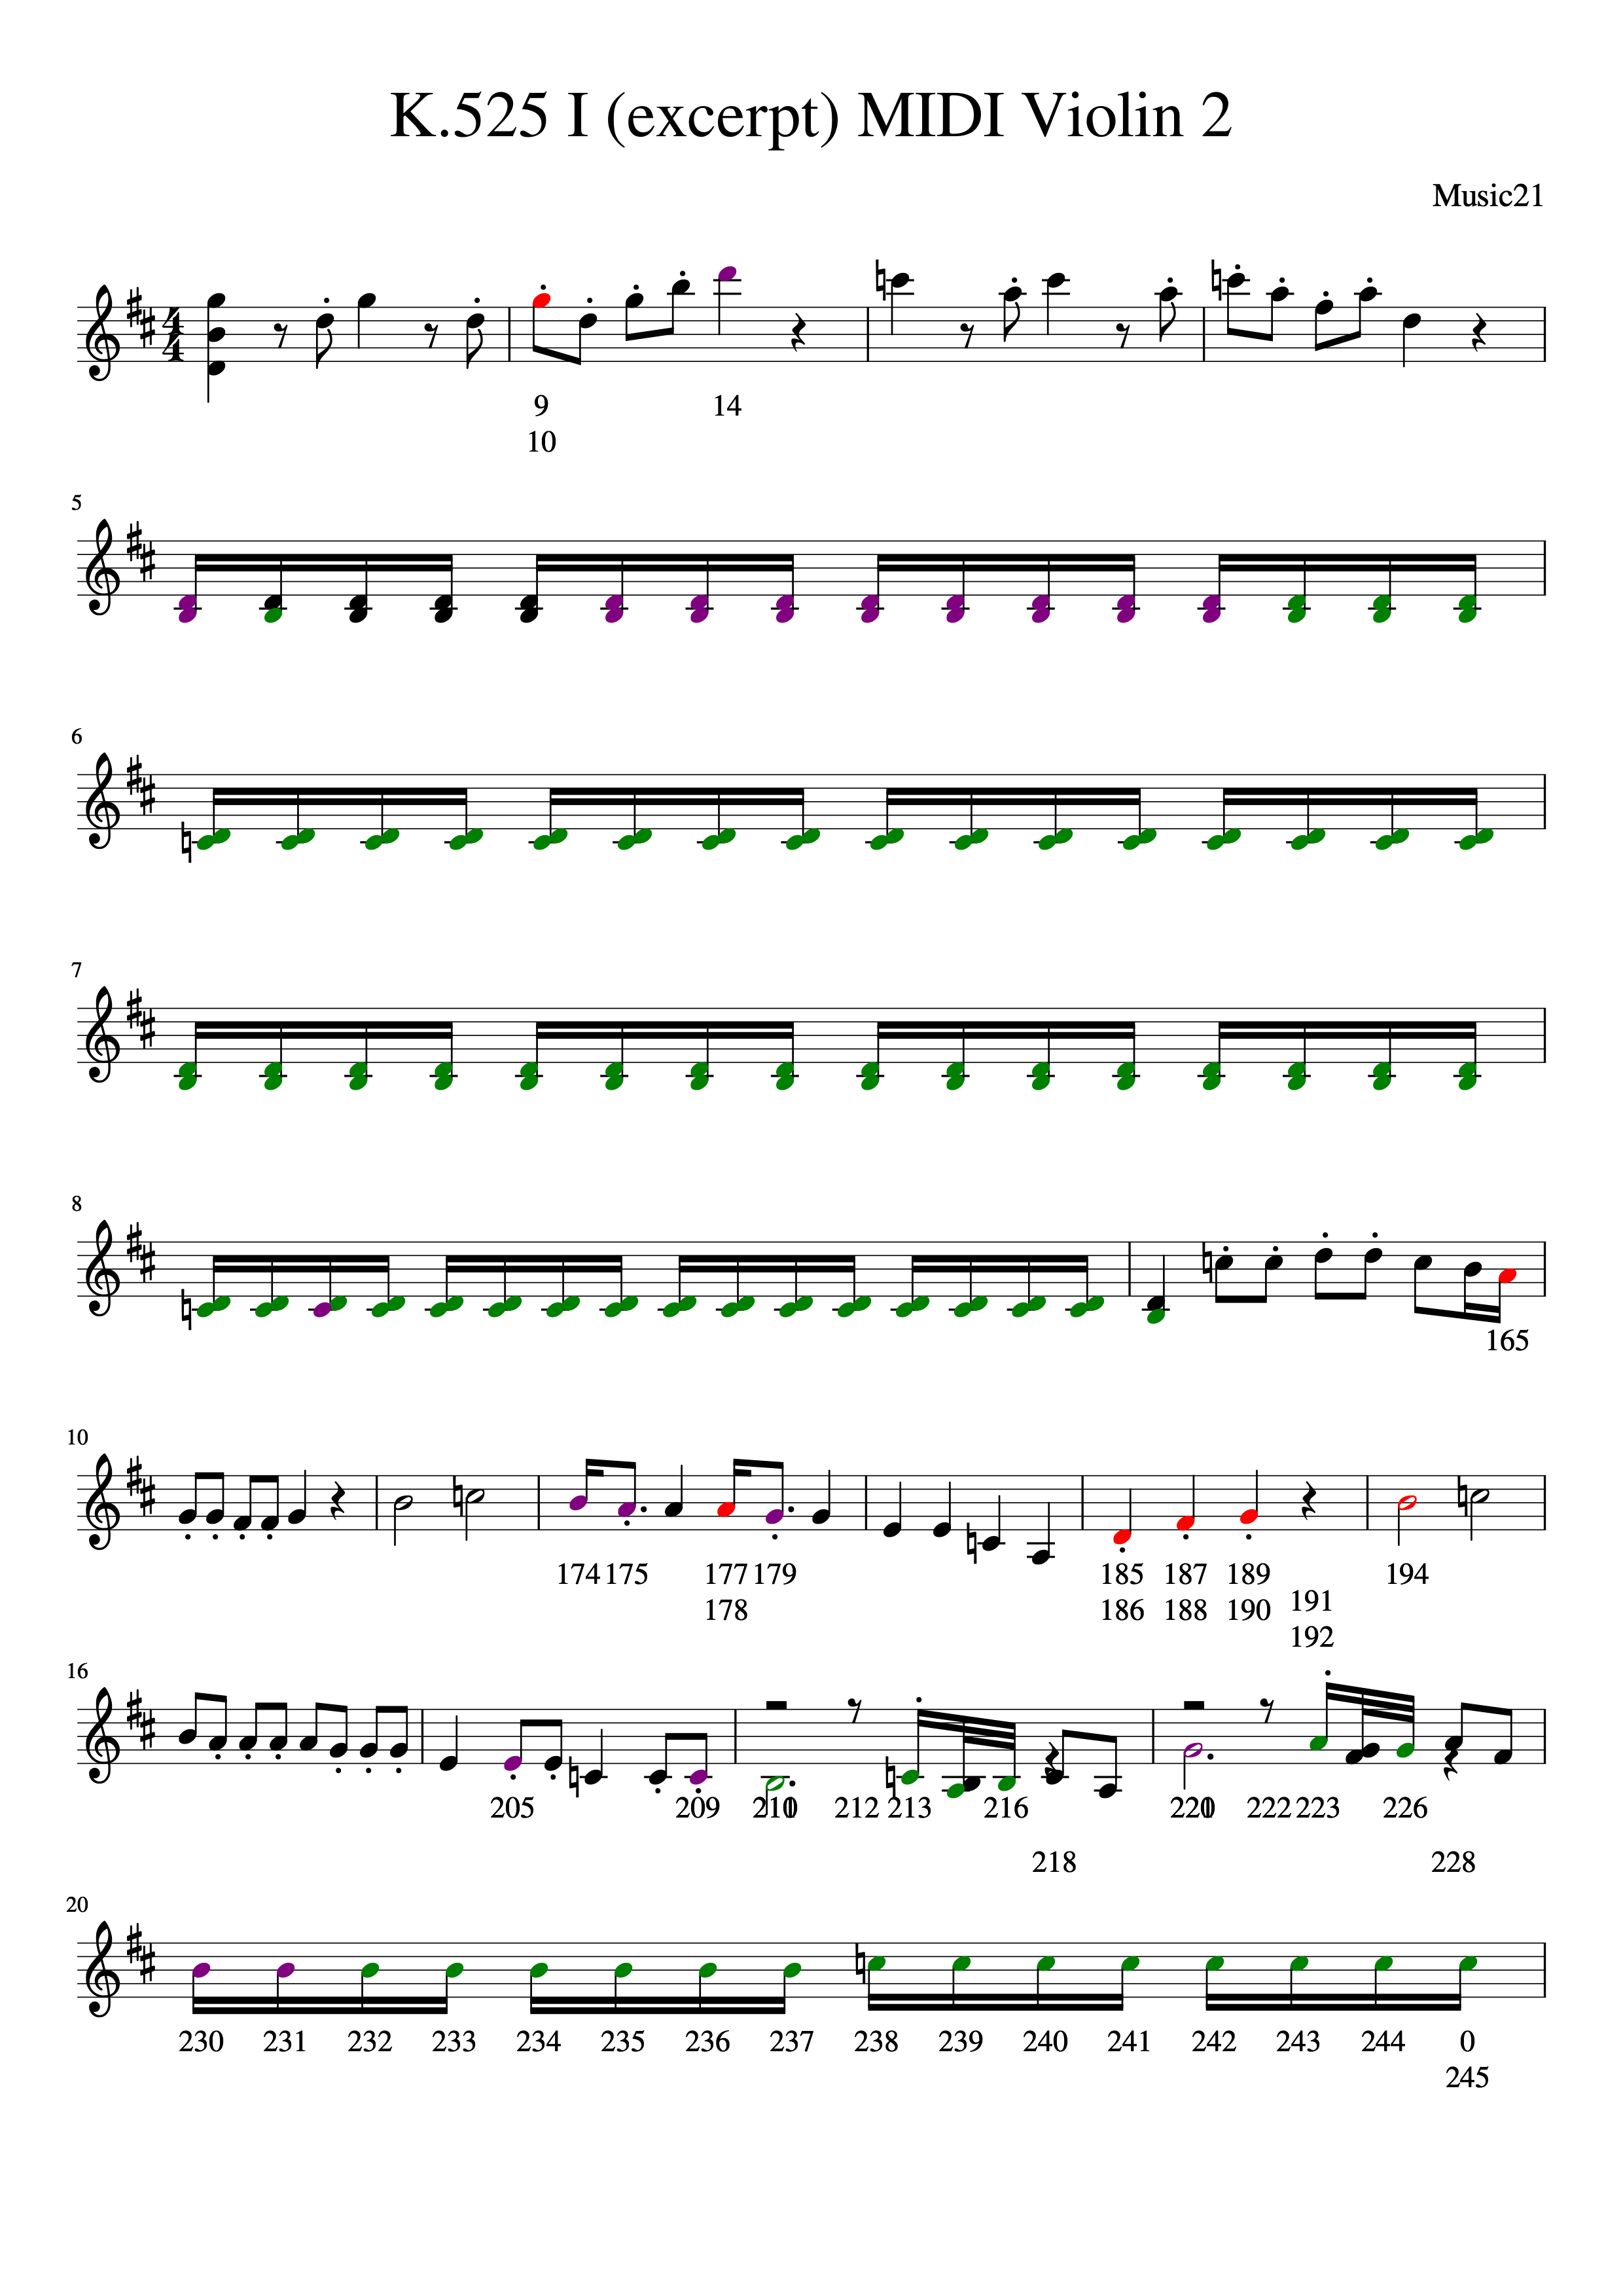
\includegraphics[width =.95\textwidth]{K525_I_MIDI_Violin_2-1}
\caption{Visual display of changes in Violin 1 of target (MIDI) stream.}
\end{figure}

\begin{figure}[H]
\centering
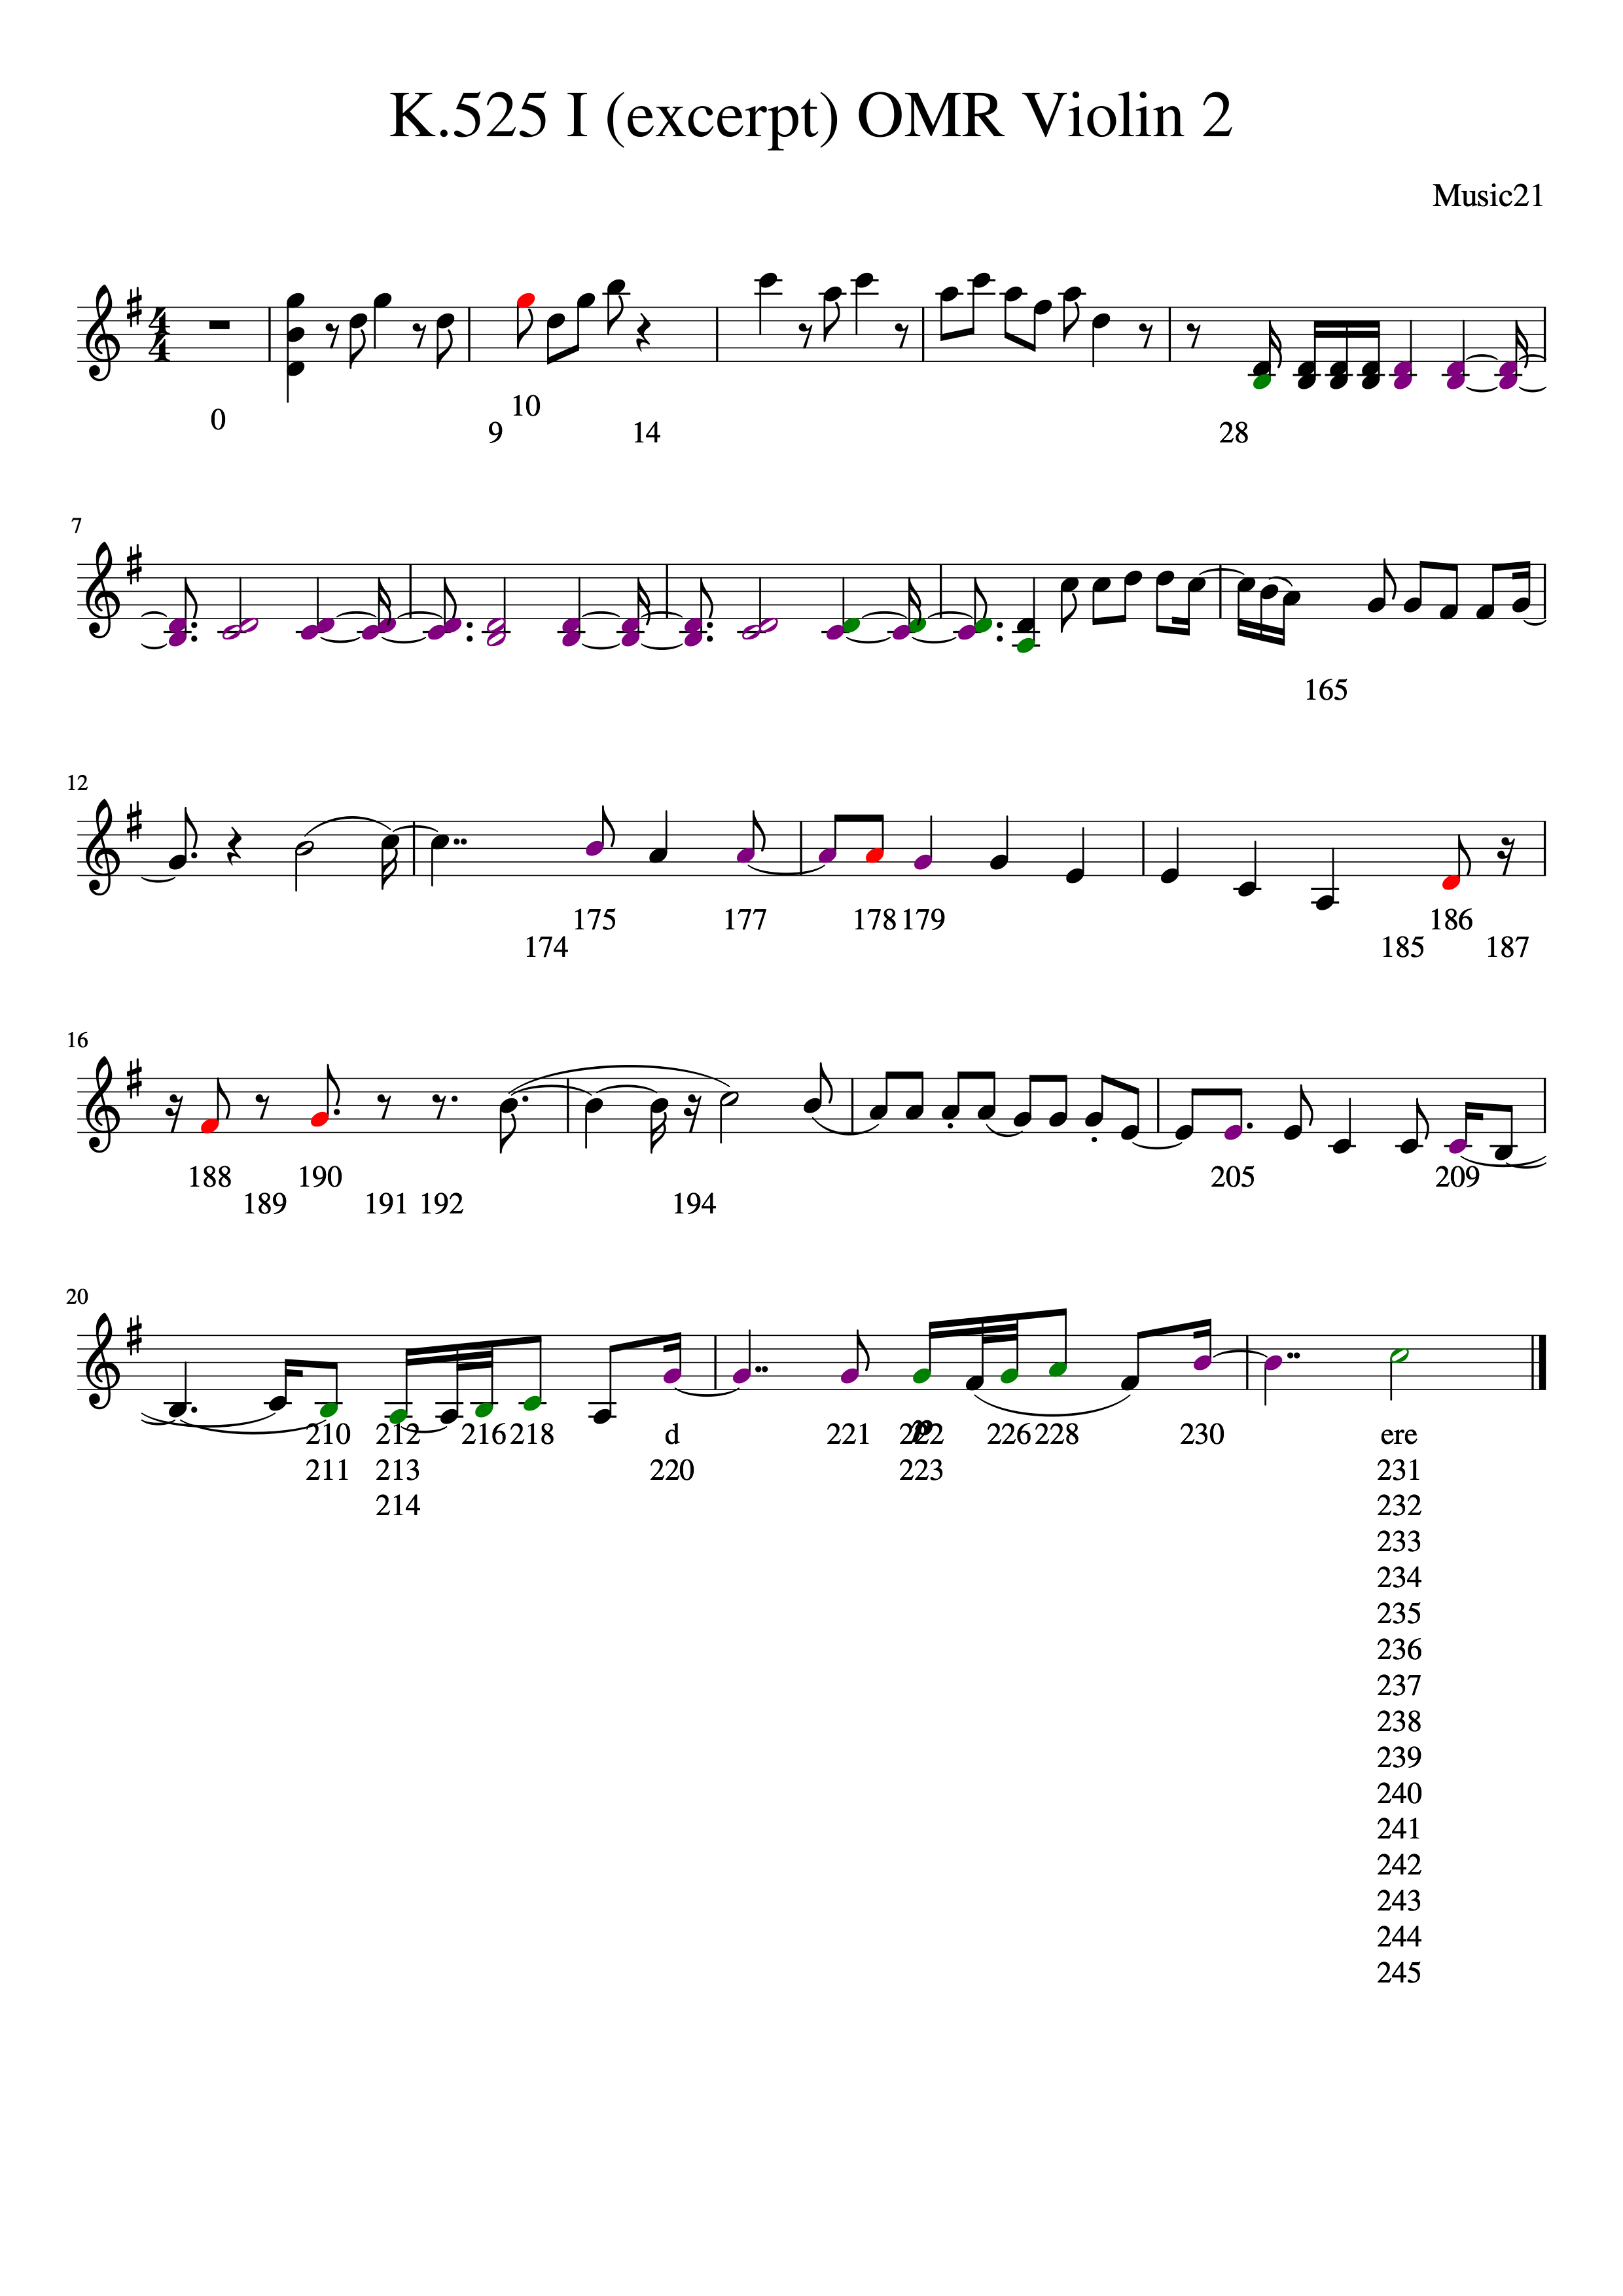
\includegraphics[width =.95\textwidth]{K525_I_OMR_Violin_2-1}
\caption{Visual display of changes in Violin 1 of source (OMR) stream.}
\end{figure}



\clearpage
\newpage

\chapter{Figures}

\vspace*{-3in}

\begin{figure}
\vspace{2.4in}
\caption{}
\label{sample1}
\end{figure}
\clearpage
\newpage

\begin{figure}
\vspace{2.4in}
\caption{}
\label{sample2}
\end{figure}
\clearpage
\newpage

%% This defines the bibliography file (main.bib) and the bibliography style.
%% If you want to create a bibliography file by hand, change the contents of
%% this file to a `thebibliography' environment.  For more information 
%% see section 4.3 of the LaTeX manual.
\begin{singlespace}
\bibliography{main}
\bibliographystyle{plain}
\end{singlespace}

\end{document}

